\documentclass[a4paper,11pt,oneside,titlepage,openright]{book}
\usepackage[english]{babel}
\usepackage[utf8]{inputenc}
\usepackage{indentfirst}
\usepackage[dvips]{graphicx}
\usepackage{amssymb}
\usepackage{amsmath}
\usepackage{latexsym}
\usepackage{amsthm}
\usepackage{mathtools}
\usepackage{amsfonts}
\usepackage{lettrine}
\usepackage{epsfig}
\usepackage{hyperref}
\usepackage{graphicx}
\usepackage{color}
\usepackage{sidecap}
\usepackage{xcolor}
\usepackage{courier}
\usepackage{caption}
\usepackage{mdwlist}
\usepackage{listings}
\usepackage[T1]{fontenc}
\usepackage{booktabs}
\usepackage{longtable}
\usepackage{pdflscape}
\usepackage{rotating}
%\usepackage[babel]{csquotes}
\usepackage{epigraph}
\usepackage{tabularx}
\usepackage[style=numeric-comp,useprefix,hyperref,backend=bibtex]{biblatex}

\bibliography{tex_files/bibliography/bibliography}
\pagestyle{headings}

\definecolor{editorGray}{rgb}{0.95, 0.95, 0.95}
\definecolor{editorOcher}{rgb}{1, 0.5, 0} % #FF7F00 -> rgb(239, 169, 0)
\definecolor{editorGreen}{rgb}{0, 0.5, 0} % #007C00 -> rgb(0, 124, 0)
\colorlet{punct}{red!60!black}
\definecolor{background}{HTML}{F5F5F5}
\definecolor{delim}{RGB}{20,105,176}
\colorlet{numb}{magenta!60!black}

\lstdefinelanguage{javascript}{
  morekeywords={typeof, new, true, false, catch, function, return, null, catch, switch, var, if, in, while, do, else, case, break},
  morecomment=[s]{/*}{*/},
  morecomment=[l]//,
  morestring=[b]",
  morestring=[b]'
}

\lstset{%
    % Basic design
    backgroundcolor=\color{background},
    basicstyle={\scriptsize\ttfamily},
    frame=none,
    % Line numbers
    numbers=none,
    % xleftmargin={0.75cm},
    % numbers=left,
    % stepnumber=1,
    % firstnumber=1,
    % numberfirstline=true,
    % Code design
    keywordstyle=\color{black}\bfseries,
    commentstyle=\color{darkgray}\ttfamily,
    ndkeywordstyle=\color{gray}\bfseries,
    stringstyle=\color{black},
    % Code
    language=html,
    alsolanguage=javascript,
    alsodigit={.:;},
    tabsize=2,
    showtabs=false,
    showspaces=false,
    showstringspaces=false,
    extendedchars=true,
    breaklines=true,
    % Support for German umlauts
    literate=%
    {Ö}{{\"O}}1
    {Ä}{{\"A}}1
    {Ü}{{\"U}}1
    {ß}{{\ss}}1
    {ü}{{\"u}}1
    {ä}{{\"a}}1
    {ö}{{\"o}}1
}

\lstdefinelanguage{json}{
    basicstyle=\scriptsize\ttfamily,
    % Line numbers
    numbers=none,
    frame=none,
    % numbers=left,
    % numberstyle=\scriptsize,
    % stepnumber=1,
    % numbersep=8pt,
    % showstringspaces=false,
    % breaklines=true,
    % frame=lines,
    backgroundcolor=\color{background},
    literate=
     *{0}{{{\color{numb}0}}}{1}
      {1}{{{\color{numb}1}}}{1}
      {2}{{{\color{numb}2}}}{1}
      {3}{{{\color{numb}3}}}{1}
      {4}{{{\color{numb}4}}}{1}
      {5}{{{\color{numb}5}}}{1}
      {6}{{{\color{numb}6}}}{1}
      {7}{{{\color{numb}7}}}{1}
      {8}{{{\color{numb}8}}}{1}
      {9}{{{\color{numb}9}}}{1}
      {:}{{{\color{punct}{:}}}}{1}
      {,}{{{\color{punct}{,}}}}{1}
      {\{}{{{\color{delim}{\{}}}}{1}
      {\}}{{{\color{delim}{\}}}}}{1}
      {[}{{{\color{delim}{[}}}}{1}
      {]}{{{\color{delim}{]}}}}{1},
}

\DeclareCaptionFont{white}{\color{white}}
\DeclareCaptionFormat{listing}{\colorbox[cmyk]{0.43, 0.35, 0.35,0.01}{\parbox{\textwidth}{\hspace{12pt}#1#2#3}}}
\captionsetup[lstlisting]{format=listing,labelfont=white,textfont=white, singlelinecheck=false, margin=0pt, font={bf,footnotesize}}

\definecolor{lightgray}{rgb}{.9,.9,.9}
\definecolor{darkgray}{rgb}{.4,.4,.4}
\definecolor{purple}{rgb}{0.65, 0.12, 0.82}
\definecolor{Brown}{cmyk}{0,0.81,1,0.60}
\definecolor{OliveGreen}{cmyk}{0.64,0,0.95,0.40}
\definecolor{CadetBlue}{cmyk}{0.62,0.57,0.23,0}
\definecolor{lightlightgray}{gray}{0.9}

\linespread{1.0}

\newcommand{\minisizeurl}[1]{\footnotesize #1 \normalsize}

\newcommand{\terminale}{
    \lstset{language={}}
}

\newcommand{\javascript}{
    \lstset{
    language=JavaScript,
    backgroundcolor=\color{lightgray},
    extendedchars=true,
    basicstyle=\footnotesize\ttfamily,
    showstringspaces=false,
    showspaces=false,
    tabsize=2,
    breaklines=true,
    showtabs=false,
    captionpos=b
   }
}

\newcommand{\html}{
    \lstset{
        language=HTML,
        basicstyle=\ttfamily\footnotesize,
        keywordstyle=\color{OliveGreen},
        commentstyle=\color{gray},
        stepnumber=1,
        numbersep=5pt,
        backgroundcolor=\color{lightgray},
        frame=none,
        tabsize=2,
        captionpos=b,
        breaklines=true,
        breakatwhitespace=false,
        showspaces=false,
        showtabs=false,
        stringstyle=\color{red}\ttfamily,
        xleftmargin=17pt,
        framexleftmargin=17pt,
        framexrightmargin=5pt,
        framexbottommargin=4pt,
    }
}

\newcommand{\xml}{
    \lstset{
        language=XML,
        basicstyle=\ttfamily\footnotesize,
        keywordstyle=\color{OliveGreen},
        commentstyle=\color{gray},
        stepnumber=1,
        numbersep=5pt,
        backgroundcolor=\color{lightgray},
        frame=none,
        tabsize=2,
        captionpos=b,
        breaklines=true,
        breakatwhitespace=false,
        showspaces=false,
        showtabs=false,
        stringstyle=\color{red}\ttfamily,
        xleftmargin=17pt,
        framexleftmargin=17pt,
        framexrightmargin=5pt,
        framexbottommargin=4pt,
    }
}

\newcommand{\ext}{png}

% \newcommand{\def}[1]{{\em {\bfseries #1}}}

\hyphenation{sil-la-ba-zio-ne}
\hyphenation{del-le} \hyphenation{pa-ro-le}

% examples
\theoremstyle{plain}
\newtheorem{thm}{Teorema}[section]
\theoremstyle{definition}
\newtheorem{defn}{Definizione}[chapter]
\newtheorem{ex}{Esempio}[chapter]
\theoremstyle{remark}
\newtheorem{codifica}{Codifica}

\begin{document}

\baselineskip=12mm
\thispagestyle{empty}

\begin{figure}
\begin{center}
~~\centerline {
\psfig{file=images/logo/logo.png,width=5cm}}
\end{center}
\end{figure}

\vskip 1.40cm

\begin{center}
\large
Università degli Studi \textit{``Roma Tre''}\\
Facoltà di Ingegneria\\
Corso di Laurea Magistrale in Ingegneria Informatica\\
\end{center}

\vskip 1cm \Large

\begin{center}
Tesi di laurea magistrale
\end{center}

\vskip 1cm \baselineskip=10mm

\begin{center}
\textbf{{\em X-commerce: Web platform to build single page e-commerce application based on HTML5 Web Components}}\\
\end{center}

\vskip .4cm

\begin{center}
Laureando\\
{Baljinder Jit}\\
\end{center}

\vskip 1cm

\begin{center}
\large{
\begin{tabularx}{\textwidth}{>{\centering\arraybackslash}X >{\centering\arraybackslash}X}
  Relatore\\
  Prof. Alberto Paoluzzi\\
\end{tabularx}
}
\large{
\begin{tabularx}{\textwidth}{>{\centering\arraybackslash}X >{\centering\arraybackslash}X}
  Co-relatore\\
  Dott. Enrico Marino\\
\end{tabularx}
}
\end{center}

\vskip 1.5cm

\centerline{Anno Accademico 2014/2015}

\normalsize


\newpage

\newpage\null\thispagestyle{empty}\newpage
\thispagestyle{empty}
\begin{flushright}
\null\vspace{\stretch{1}}
{\em Dedicated to my family} \\
\vspace{\stretch{2}}\null
\end{flushright}

\frontmatter

\tableofcontents

\listoffigures

\chapter{Acknowledgements}
\label{cha:acknowledgements}

Thanks to...


\chapter{Introduction}
\label{cha:introduction}

Today, the Electronic Commerce has changed the way we shop, Internet, in fact, has become a valuable communication tool for the enterprise network.
The company, through the website, is able to provide you with a communication and customized promotion, personalized offer, a transaction customized, personalized assistance. Enter the network, it means coming to terms everyday, with the global market, the global consumer, competition global; to remain in the competition and gain greater visibility the company must adopt a new sales channel: e-commerce.
\newline
Electronic commerce is one of the main criteria of revolution of Information Technology and communication in the field of economy. Existence of this virtual markets, passages and stores that have not occupy any physical space, allowing access and circulation in these markets for a moment and anywhere in the world without leaving home is possible. Select and order goods that are placed in virtual shop windows at unspecified parts of the world and also are advertising on virtual networks and payment is provided through electronic services, all of these options have been caused that electronic commerce is considered the miracle of our century.
\newline
\begin{figure}[htb]
 \centering
 
\includegraphics[width=1.0\linewidth]{images/introduction/ecommerce-wordle.jpg}\hfill
 \caption[e-commerce wordle]{e-commerce wordle}
 \label{fig:e_commerce_wordle}
\end{figure}
The increased availability of Internet access and the wide spread of mobile devices has allowed us to consolidate the habit of buying online by customers online already active, that have increased the share of online spending on total consumption.
But what is the correct definition of e-commerce?
\newline
“Commerce is the activity of buying and selling of goods and services, especially on a large scale. The system includes legal, economic, political, social, cultural and technological systems that are in operation in any country or internationally. Thus, commerce is a system or an environment that affects the business prospects of economies. It can also be defined as a component of business which includes all activities, functions and institutions involved in transferring goods from producers to consumers \cite{commerce_def_1}.”
\newline
Other definition:
“Interaction between communication systems, data management systems and security, which because of them exchange commercial information in relation to the sale products or services, will be available, so the definition, the main components of electronic commerce are: communication systems, data management systems and security \cite{commerce_def_2}.”
\newline
In the 1970s, the term electronic commerce, referred to electronic data exchange for sending business documents such as purchase orders and voices electronically. Later, with the development of this industry the term of electronic commerce is used to business of goods and services via the web. When the first World Wide Web was introduced in 1994 as a comprehensive, many well-known researchers have been predicated this type of business “the web-based business” will became soon an important in the world economy, but it took four years that http based protocols should be widely available to users.
The aim of this thesis either to analyze the main systems of e-commerce platforms and either facilitating their realization.
 \newline
Therefore, this thesis is divided in two parts and organized as follows:
Part one consists of five chapters. Chapter One describes the state of the art system of e-commerce and the platforms that their facilitate the realization. Chapter two, analyzes the main companies of e-commerce and the platforms that build systems. Chapter tree analyzes each technology used and describes the methodological approach of each. Fourth chapter analyzes the payment services used. Chapter five provides an overview of Single Page Application development pattern and explains pros and cons and technical functioning.
The second part consists of three chapters. Chapter five describes the project as a whole showing the structure and organization pages. Chapters six is focus on specific components that have been developed, Payment Management and on all the theorical and practical concepts that are behind the ideation of the component. Finally, Chapter seven, exposes project conclusions and further implementations of the work.

\mainmatter

\part{Part 1}
\label{part:part_1}


\chapter{Chapter 1}
\label{cha:chapter_1}

This chapter describes the main systems of e-commerce and the most popular platforms that facilitate their realization.
The first section provides an overview of e-commerce systems as Amzon, Ebay and discusses the advantages and disadvantages of such systems. Also describes the main leaders of the existing global market e-commerce systems. The second section describes in general terms the platforms that facilitate the creation of an electronic trading system and illustrates the main leading companies that offer these types of services as Shopify, BigCommerce, Prestashop.

\section{E-commerce Overview}
\label{sec:e_commerce_overview}
“Interaction between communication systems, data management systems and security, which because of them exchange commercial information in relation to the sale products or services, will be available, so the definition, the main components of electronic commerce are: communication systems, data management systems and security \cite{commerce_intro_1}.”
\newline
Today, most of the population, use these virtual stores to shop or simply to inquire. In fact, these systems allow for a timely basis to have information regarding the good we are seeking. In this way these systems help the customer in buying a particular good.
\newline
\begin{figure}[htb]
 \centering
 
\includegraphics[width=0.8\linewidth]{images/chapter1/e-commerce.png}\hfill
 \caption[e-commerce overview]{e-commerce overview}
 \label{fig:e_commerce_overview}
\end{figure}
The e-commerce in Europe has continued to grow even if at different rates and in different ways in different countries.
The Commission's Digital Agenda for Europe aims to get 50\% of all European citizens to buy online and 20\% to engage in online cross-border transactions by 2015. The communication “Building trust in the Digital Single Market for ecommerce” (European Commission, 2012) proposed measures to boost online retail trade in the EU and overcome obstacles to e-commerce. These obstacles include an insufficient number of online shops willing to sell across the border, inadequate payment and parcel delivery systems, and too many cases of abuse and disputes that are difficult to settle \cite{e_commerce_eu}.
\newline
Online shopping is a habit well established in Britain, Germany and France, markets that together account for 70-80\% of e-commerce Europe, while it is just starting out or is growing in the rest of Europe, including countries such as Italy and Spain. The most rapid growth, however, affect the emerging economies of Eastern Europe, led by Russia, the market for which is expected to grow by up to 200\% over the next three years.
\newline
In mature markets, growth was driven primarily by an increase in the frequency of purchase by the consumer and by the tendency to spend more through online channels, while in countries where e-commerce is developing growth results especially by the increase in online shoppers \cite{e_commerce_in_italy}.
\newline
The cellphone is the key factor in the growth of e-commerce. The diffusion of smartphones and tablets has extended much access to the online market, even in Italy, where 29 million end users access the Internet from the mobile. Companies that have not addressed this change have had a decline in the conversion rate on its website, while those who understood the new opportunities brought by the new type of access has been able to develop the offer of additional products and services dedicated, for example taking advantage of the geolocation of the customer. New entrants are mainly the physical stores, which saw in e-commerce for a way to expand its customer base, and producers of goods and services, they see the distribution companies increasingly as an obstacle to profitability.
\newline
What are the advantages and disadvantages (risks) of a system of e-commerce?
\subsection{Advantages and disadvantages of a system of e-commerce}
The benefits of electronic commerce are general (system-wide) and specific for the seller or the buyer.
\begin{itemize}
  \item Benefits for system:
  \begin{itemize}
    \item It is a global phenomenon and that a potentially global market;
    \item the transactions can develop throughout the day without interruption and realtime;
    \item the interaction between the parties can be synchronous or asynchronous;
    \item there is greater operational flexibility of relations between the parties.
  \end{itemize}

  \item Benefits for buyer:
  \begin{itemize}
    \item \emph{comfort}: e-commerce stores are always open every day including holidays: just a few clicks from home or from work to buy what you want. The convenience to receive the goods directly at home is an important added value: we forget the long lines in the parking lot and in front of the chest of the crowded malls and you live a better buying experience;
    \item \emph{convenience}: a purchase through the Web is much more convenient. In addition to the discounts and promotions who flock the network there is convenience in movement (no need to move by car or public services) and in the time saved;
    \item \emph{information}: buying on the Internet allows you to calmly assess the choice of major purchases due to the large amount of information that you can easily find, to the advice and comments from other consumers, the wide range of products and alternatives;
  \end{itemize}
  \item Benefits for seller:
    \begin{itemize}
    \item the \emph{flexibility} according to your needs of its commitments is easy to plan a few hours each day to devote to a new major project sales with the Internet. The mailbox collects communications and orders will be processed as soon as possible;
    \item \emph{visibility}: there is no place in the world frequented the Internet, after an initial phase of advertising the same managers are surprised of the amount of visits and contacts received. Those who already have a business and want to open a new sales channel with the Internet, should not overlook the excellent positive return in terms of image that the site produces and that also benefits traditional activity;
    \item the \emph{economy}: starting a new project sales with Internet does not require large investments and for the creation of storefront, both for advertising, both for the organization. Furthermore a good design e-commerce based on appropriate contacts with the suppliers allows to reduce to a minimum investment of stock.
  \end{itemize}
\end{itemize}
Companies that sell products or services on the Internet to be successful must obtain credibility and visibility on the Web and to achieve this it is not enough to have a secure server. To get credibility, companies need to know how to build for the users of their website, a positive experience not only during the purchasing process, but also before and after, so that the user wants to repeat the experience and advice to other users. Creating a positive experience for their customers and by advertising messages and techniques of SEO (Search Engine Optimization) companies build a reputation or image of successful enterprise.
\newline
In face-to-face transactions, customers and sellers use a number of physical signals to determine that they are dealing with a trustworthy partner. Retailers can check signatures and identity cards of their clients; buyers can see the badges with the name of employees, try the goods carefully and retain proof of their purchases. On electronic networks, none of these methods is applicable. For this reason, have been developed (and are now fully available and effective) some control systems performing similar functions.
\newline
The low cost of entry and the ease with which text and graphics can be copied, make it possible for almost anyone to create a website that pairs represent an organization established trading. No new reports of false virtual shops look professional, created to impersonate the Web version of existing activities, in order to illegally obtain credit card numbers. This problem has been resolved. Scammers are able to intercept transmissions. A thief can work hard to get the numbers of credit cards. A competitor or a disgruntled customer can enter an error in the company's website, in order to induce him to refuse service to potential customers or initiate other unauthorized actions. Sources intentional or accidental sometimes cause changes to the content of a communication route. User's name, credit card numbers and total currency are all vulnerable to such alteration. To this we have been developed safety systems to ensure the integrity of all the phases of the transaction. The data coming from America, are explicit: the continued growth of e-commerce is comforting. A concern, however, is the security front. In fact, the problems related to information security are increasing.
\newline
You can identify two types of Internet attacks to the network:
\begin{itemize}
  \item \emph{Passive attacks}: Need to get the most information about the network in question, but does not have the purpose of hostile intrusion; (Ex. Eavesdropping: sniffing the information being sent across it in order to acquire the contents of transactions for subsequent analysis on personal data, or on behalf of third parties);
  \item \emph{Active attacks}: as a result of the information collected by passive attacks, you can attack systems identified to implement changes to the data, lock services, obtain confidential information.\ldots
\end{itemize}
Another worrying phenomenon, in terms of information security, is surely the phishing; It is an illegal system to collect sensitive data such as information about your credit card or access to bank accounts. The vast majority of messages takes place starting from phishing e-mail addresses stolen (ie where the authors have introduced illegally) or forged to perfection (in the eyes of the end user) on the basis of a known syntax or through the use of imitators sites of companies-mirror. These threats can cause a loss of integrity of databases, a loss of profits, increased costs for security systems, a critical data loss, a loss of trade secret information and damage to corporate reputation.
\newline
The most famous e-commerce systems are Amazon, Ebay, etc.
\subsection{Amazon}
Amazon.com, Inc., often referred to as simply Amazon, is an American electronic commerce and cloud computing company with headquarters in Seattle, Washington. It is the largest Internet-based retailer in the United States \cite{amazon_wiki}.
\begin{figure}[htb]
 \centering
 
\includegraphics[width=0.4\linewidth]{images/chapter1/amazon_logo.png}\hfill
 \caption[Amazon logo]{Amazon logo}
 \label{fig:amazon_logo}
\end{figure}
Amazon.com started as an online bookstore, later diversifying to sell DVDs, Blu-rays, CDs, videodownloads/streaming, MP3 downloads/streaming, audiobook downloads/streaming, software, video games, electronics, apparel, furniture, food, toys and jewelry. The company also produces consumer electronics—notably, Amazon Kindle e-book readers, Fire tablets, Fire TV and Fire Phone - and is the world's largest provider of cloud infrastructure services (IaaS). Amazon also sells certain low-end products like USB cables under its in-house brand AmazonBasics.
\newline
Amazon has separate retail websites for United States, United Kingdom and Ireland, France, Canada, Germany, Italy, Spain, Netherlands, Australia, Brazil, Japan, China, India and Mexico.
\newline
Amazon also offers international shipping to certain other countries for some of its products. In 2011, it professed an intention to launch its websites in Poland and Sweden.
In 2015, Amazon surpassed Walmart as the most valuable retailer in the United States by market capitalization.
\newline
The company was founded in 1994, spurred by what Bezos called his “regret minimization framework,” which described his efforts to fend off any regrets for not participating sooner in the Internet business boom during that time.
\begin{figure}[htb]
 \centering
 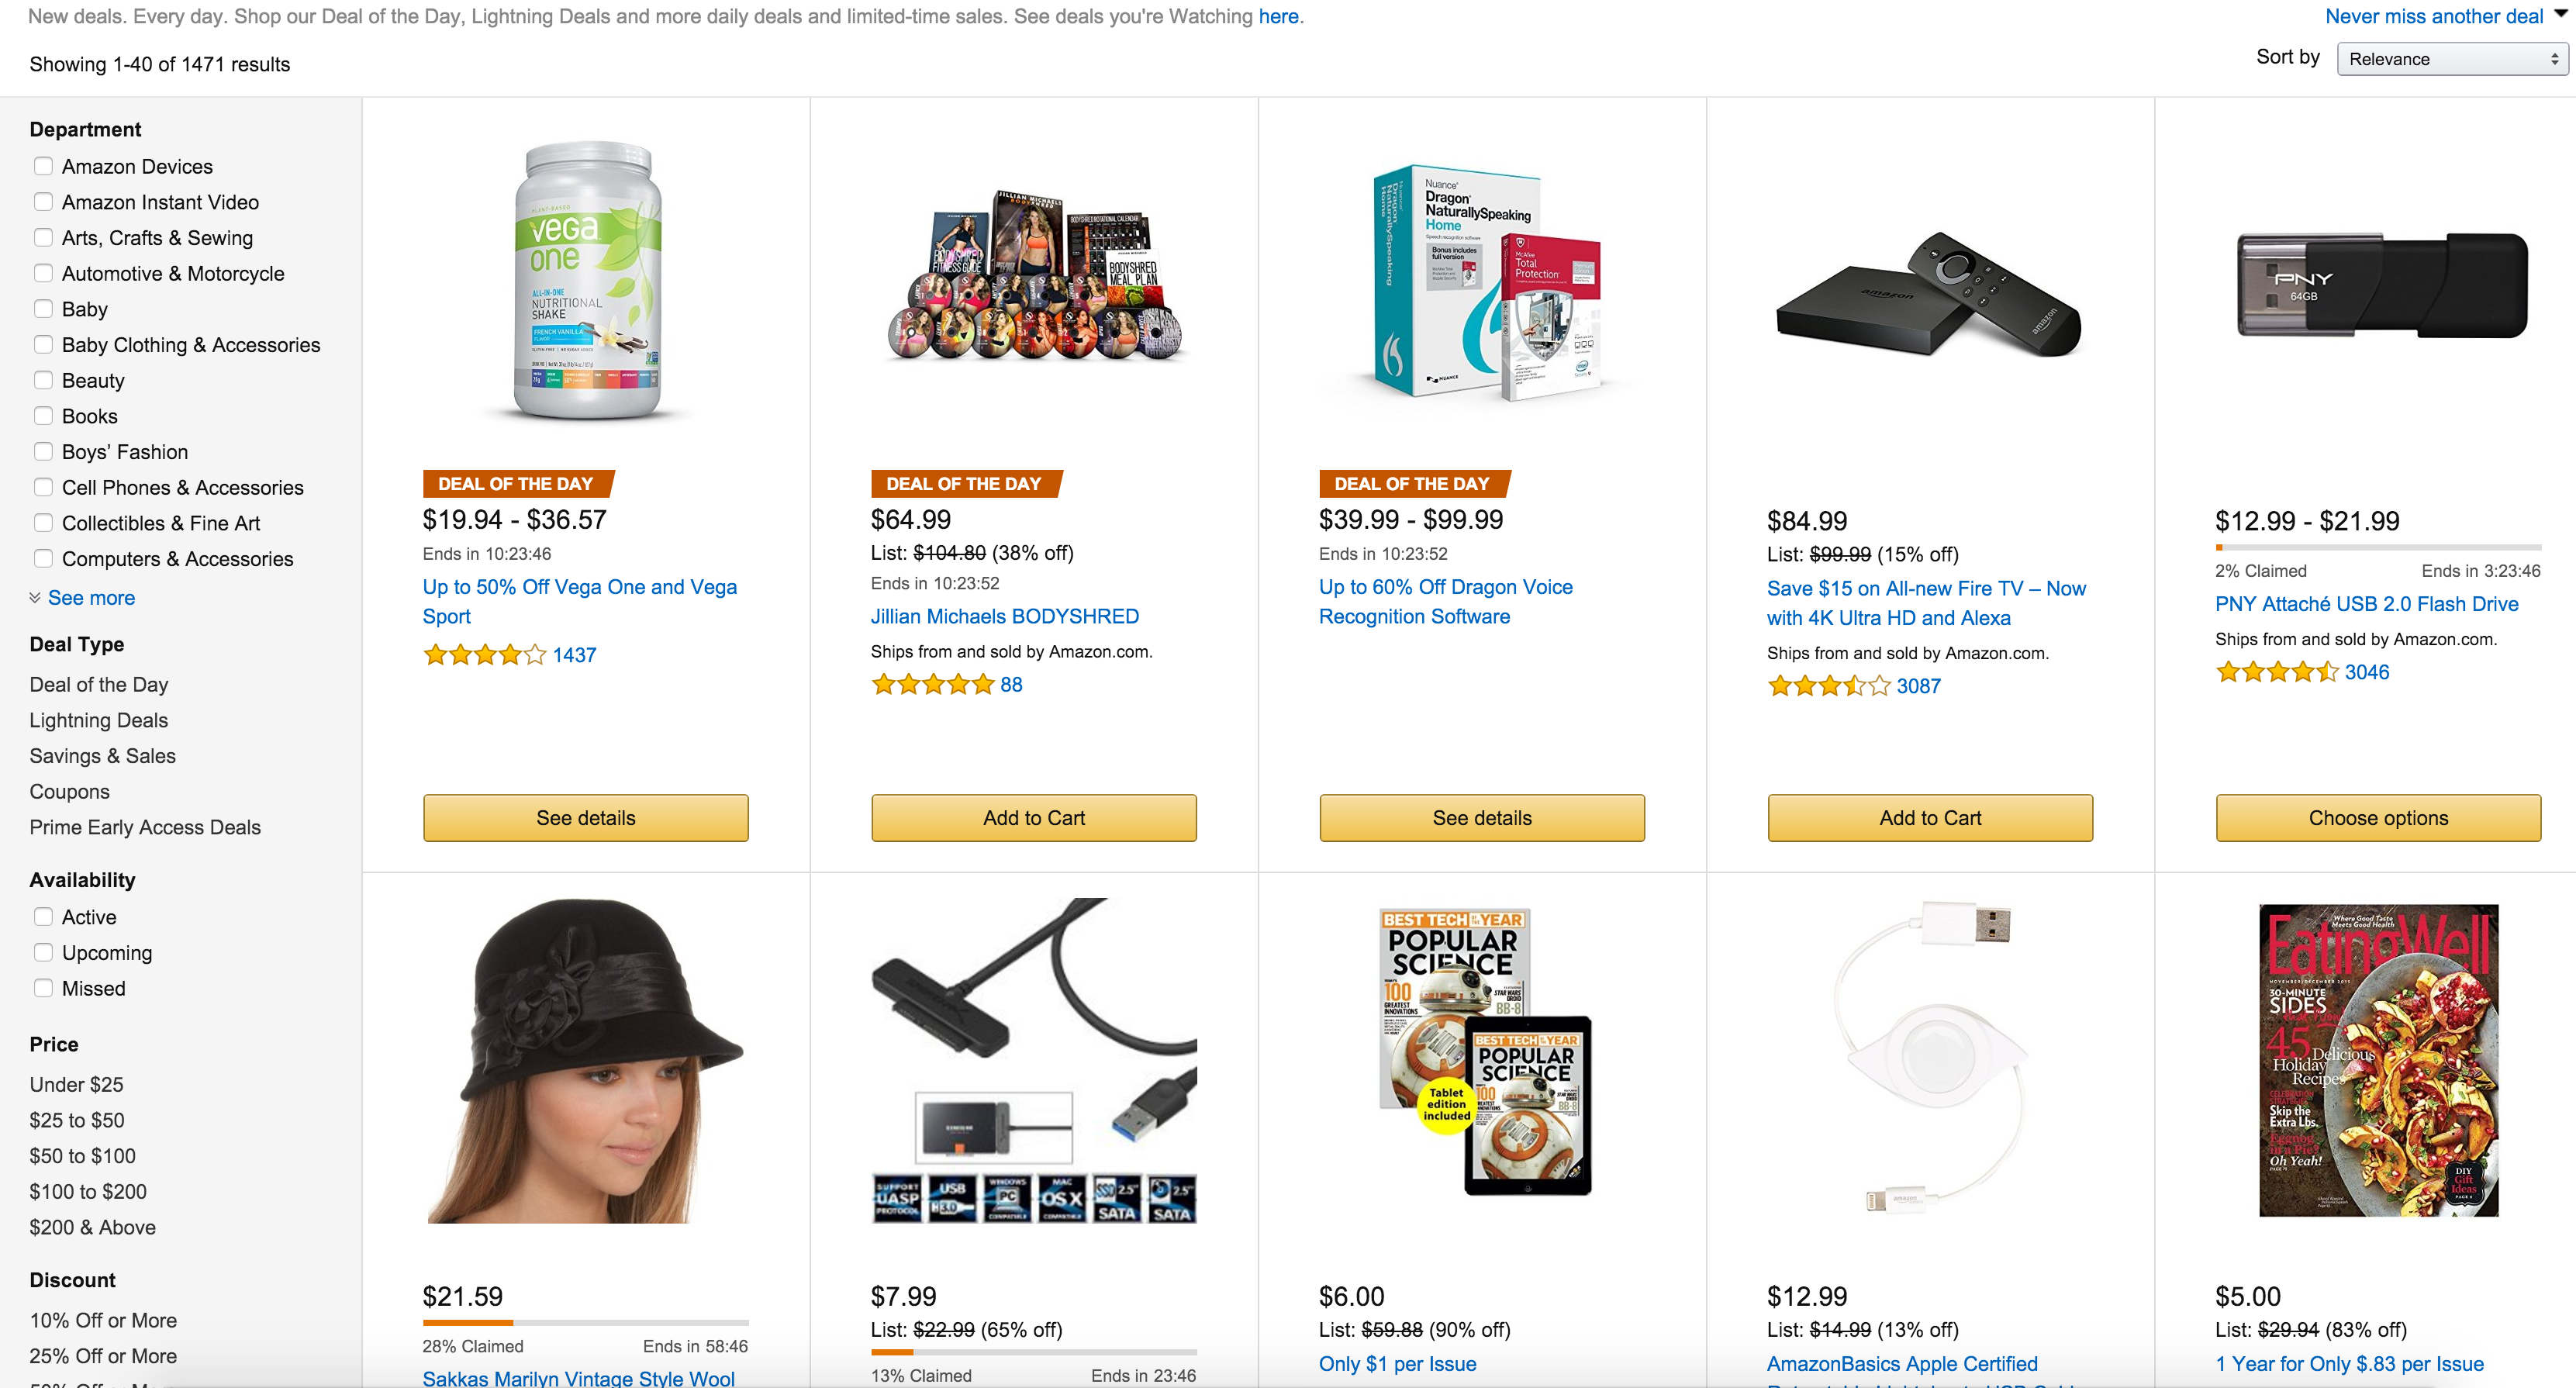
\includegraphics[width=1.0\linewidth]{images/chapter1/ex-amazon.png}\hfill
 \caption[Amazon shop]{Amazon shop}
 \label{fig:e_commerce_amazon_shop}
\end{figure}

\subsection{Ebay}
Ebay Inc. is an American multinational corporation and e-commerce company, providing consumer to consumer and business to consumer sales services via Internet \cite{ebay_wiki}.
\begin{figure}[htb]
  \centering
  
\includegraphics[width=0.3\linewidth]{images/chapter1/ebay_logo.jpeg}\hfill
  \caption[Ebay logo]{Ebay logo}
  \label{fig:ebay_logo}
\end{figure}
It is headquartered in San Jose, California. eBay was founded by Pierre Omidyar in 1995, and became a notable success story of the dot-com bubble. Today, it is a multibillion-dollar business with operations localized in over 30 countries. The company manages eBay.com, an online auction and shopping website in which people and businesses buy and sell a broad variety of goods and services worldwide. In addition to its auction-style sales, the website has since expanded to include “Buy It Now” shopping; shopping by UPC, ISBN, or other kind of SKU (via Half.com); online classified advertisements (via Kijijior eBay Classifieds); online event ticket trading (via StubHub); online money transfers (via PayPal) and other services.
\newline
The website is free to use for buyers, but sellers are charged fees for listing items and again when those items are sold. The company also makes additional money through its PayPal subsidiary which is used by sellers to collect payment for items sold.
\begin{figure}[htb]
 \centering
 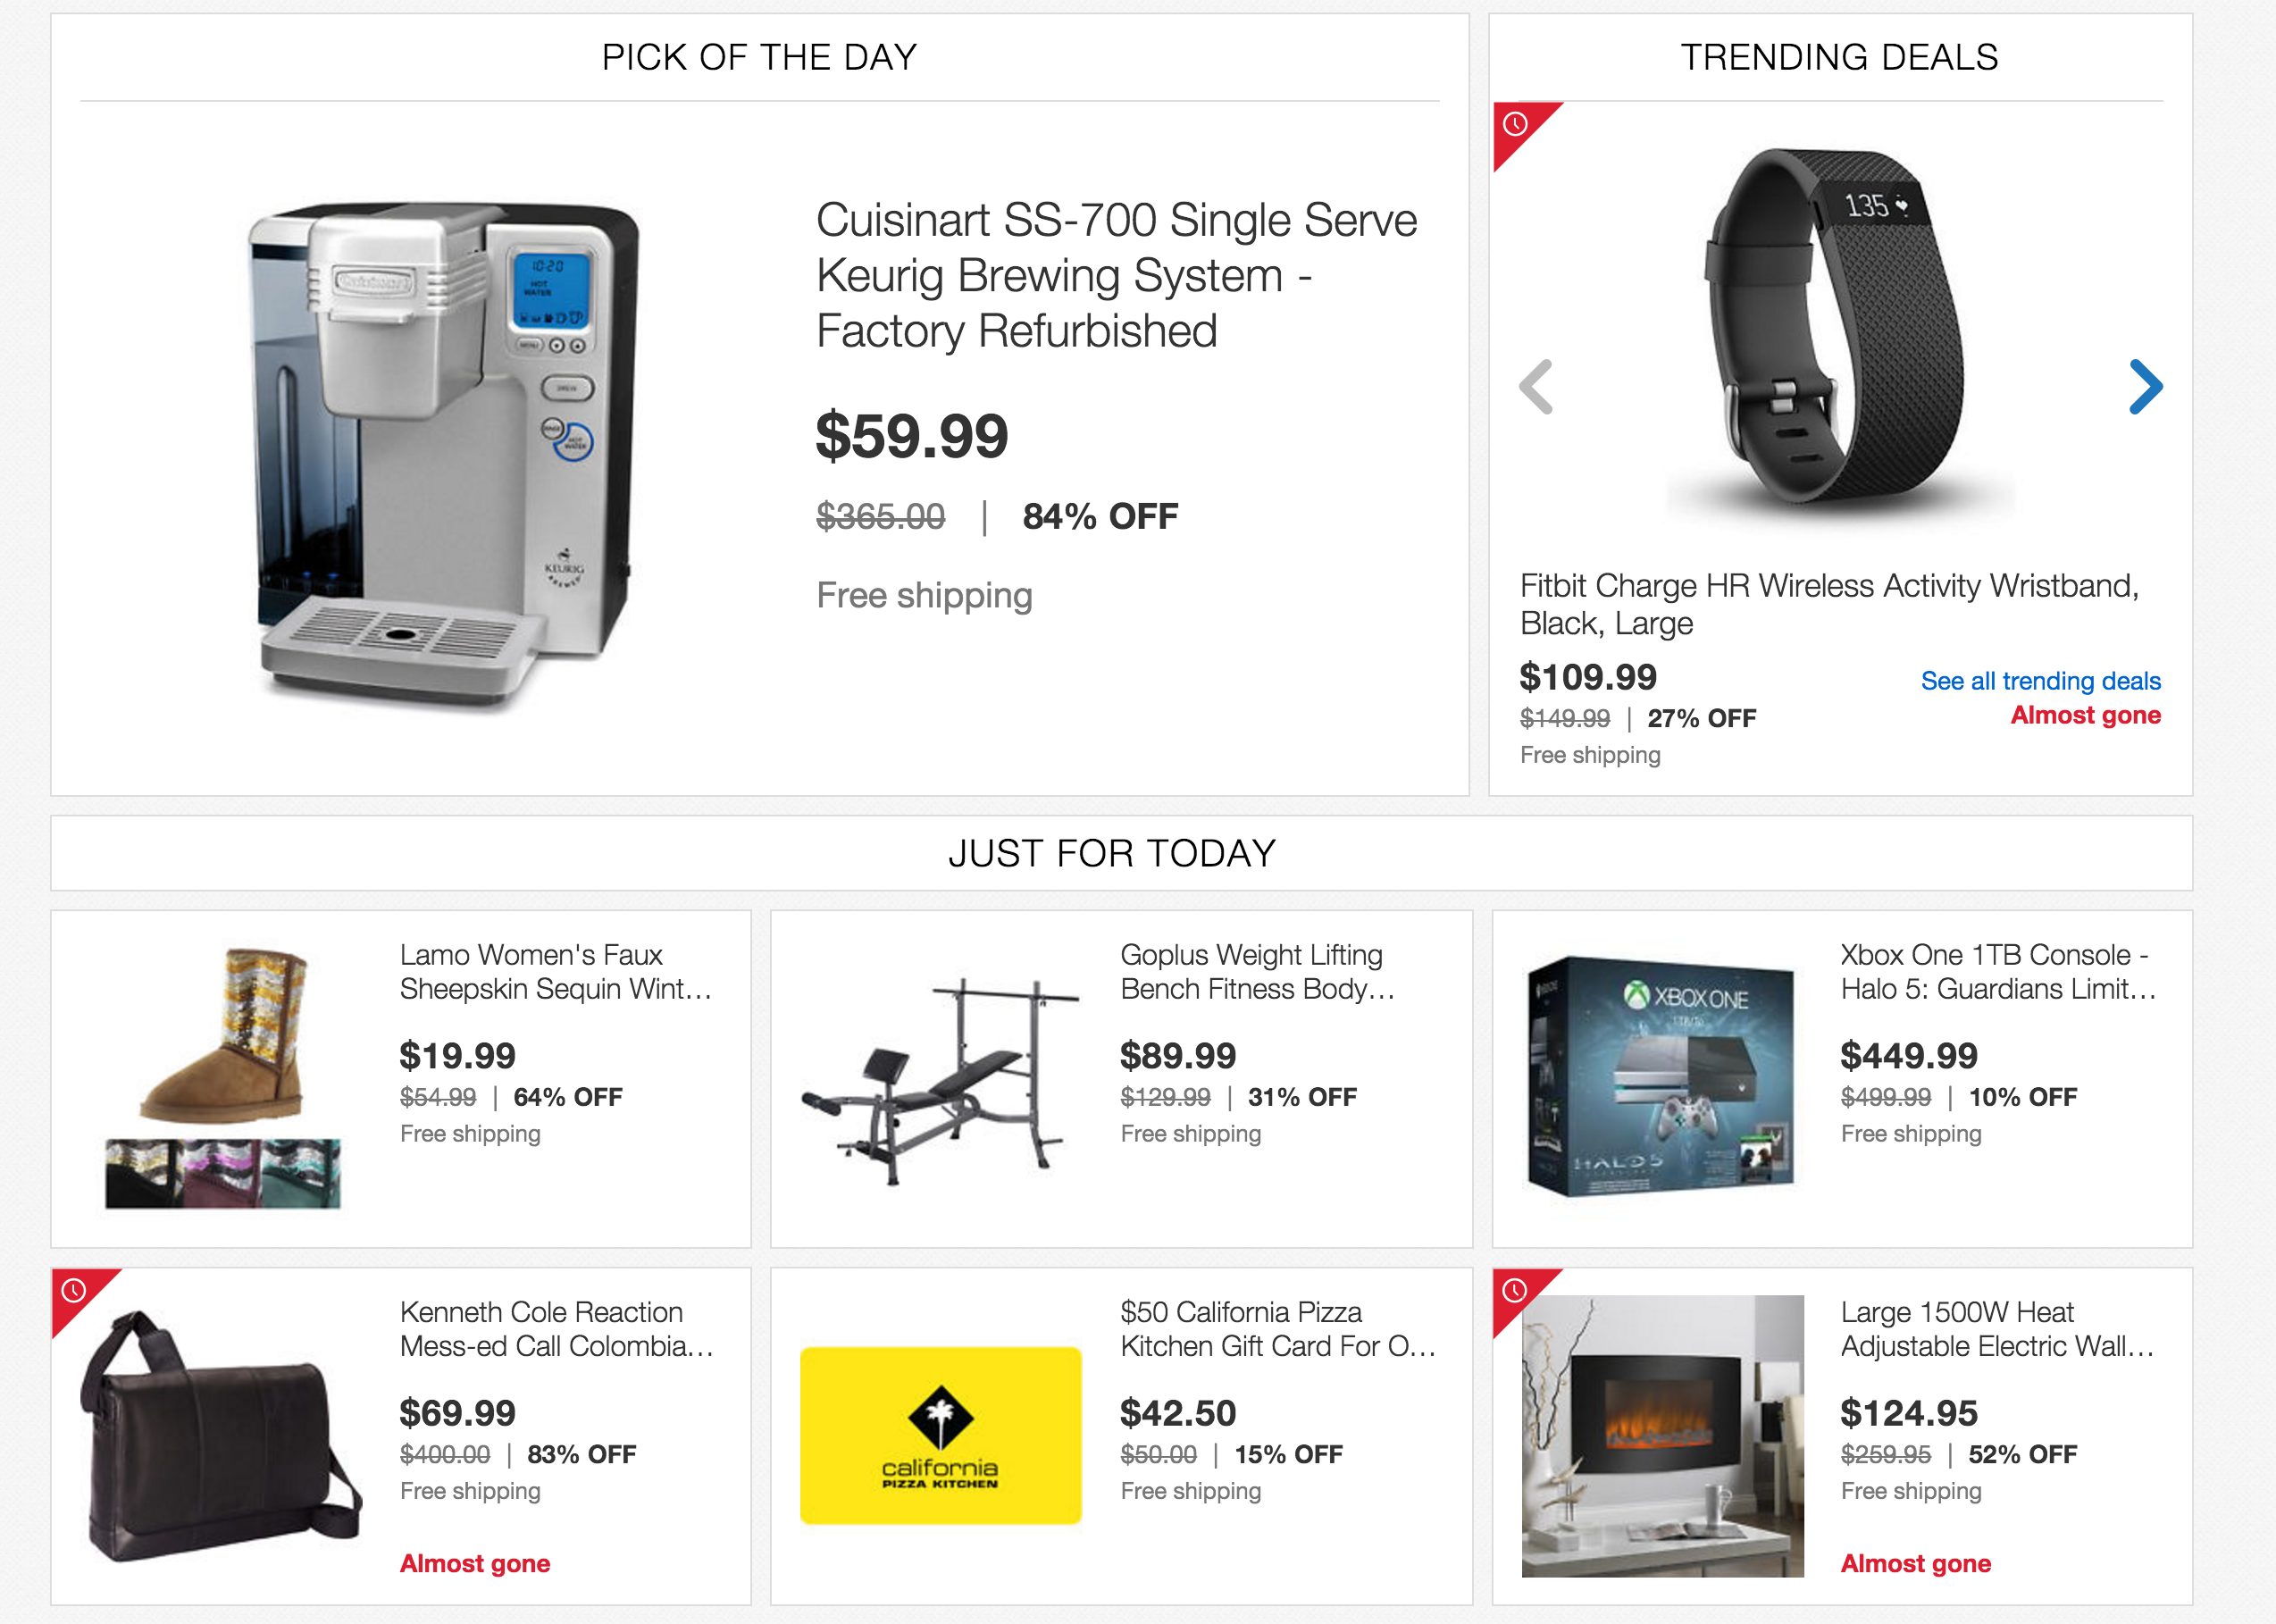
\includegraphics[width=1.0\linewidth]{images/chapter1/ex-ebay.png}\hfill
 \caption[Ebay shop]{Ebay shop}
 \label{fig:e_commerce_ebay_shop}
\end{figure}

\section{The platforms that build system of e-commerce - Overview}
\label{sec:platform_overview}
The platforms that help build a system of e-commerce are exactly systems or portals that facilitate the life of a traded that want to start your own online business.
\newline
The process of setting up an online store with such systems is very fast and efficient, because essential information is easy to fit. The next moment is the choice of the graphical presentation of the store where the trader can choose from many themes and templates available.
These systems handle transparently different services that help create the store such as: the domain, payment management, organizing inventory, shipping and tracking of shipments, invoice management, etc.
\newline
The advantages and disadvantages of these platforms are mainly linked to the flexibility of the system itself. In fact, a platform for e-commerce-rich services, has more chance of being used by a growing number of major traded.
\newline
Obviously, a generic platform so can not meet the needs of every type of merchant because the platform has the purpose of facilitating the realization of a system of e-commerce in a more simple possibilie. Therefore it is difficult to meet the needs of each merchant from any kind of detail. Ease of use is another key point that leads to the platform to be chosen by dealers.
\newline
Following is shown the shopping cart technologies used by online stores globally. Last update Feb 24th 2016 \cite{commerce_platform_comparison}.
\begin{figure}[htb]
  \centering
  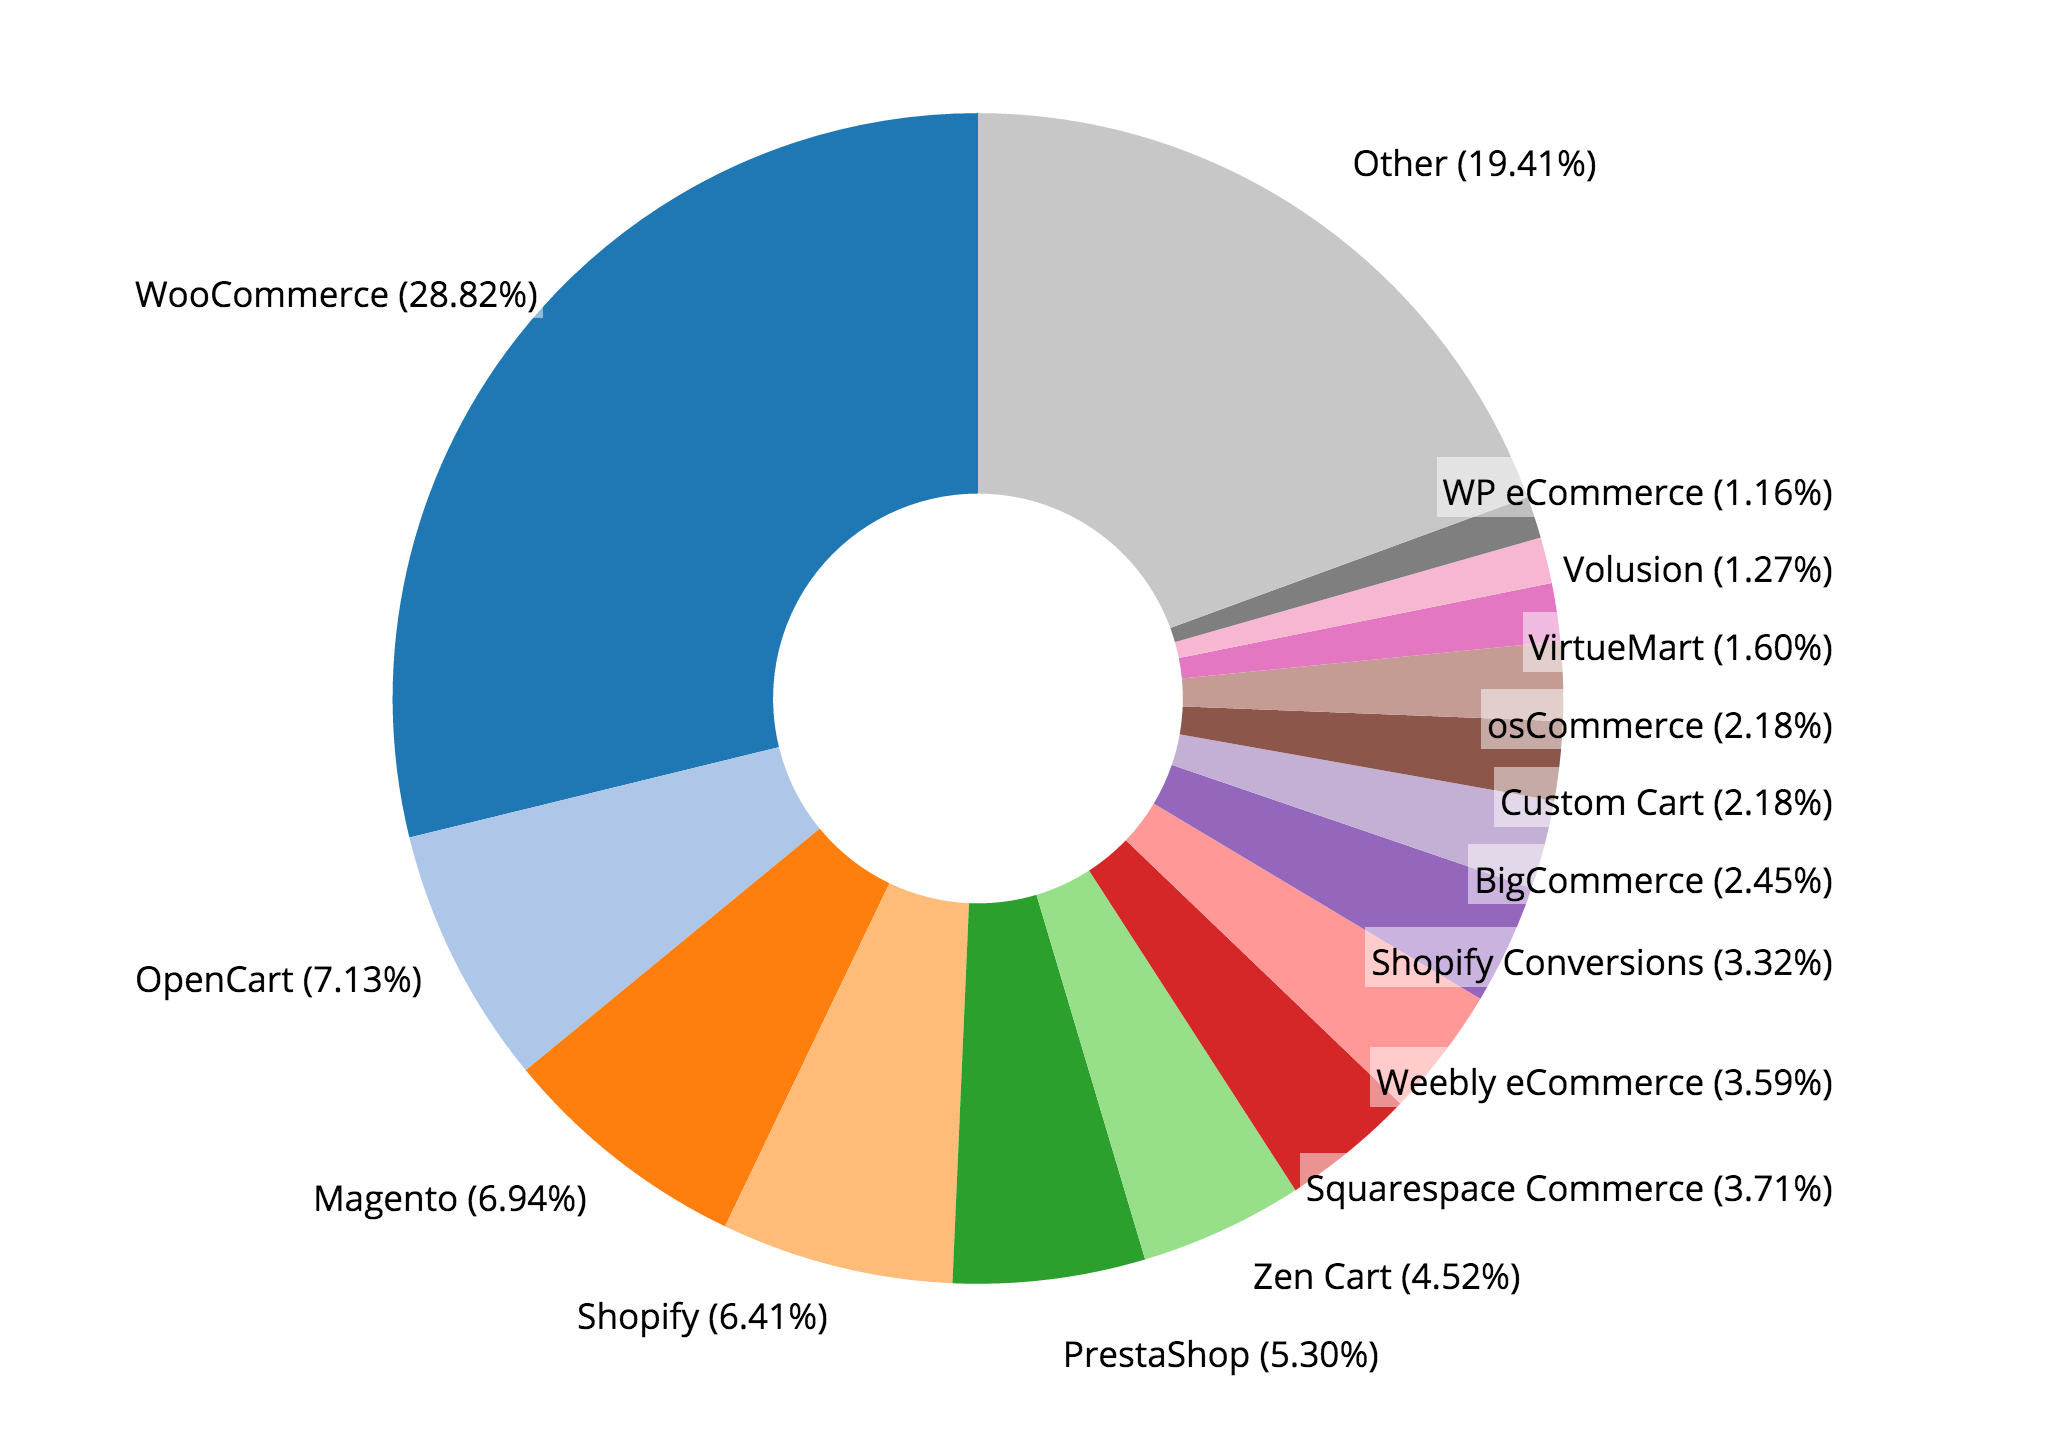
\includegraphics[width=0.8\linewidth]{images/chapter1/platform_comparison.png}\hfill
  \caption[Shopping cart technologies]{Shopping cart technologies}
  \label{fig:shopping_cart_technologies}
\end{figure}
\subsection{Shopify}
Shopify is a Canadian commerce company headquartered in Ottawa, Ontario that develops computer software for online stores and retail point-of-sale systems \cite{shopify_overview}.
\begin{figure}[htb]
  \centering
  
\includegraphics[width=0.5\linewidth]{images/chapter1/shopify_logo.png}\hfill
  \caption[Shopify logo]{Shopify logo}
  \label{fig:ebay_logo}
\end{figure}
Shopify was founded in 2004, and was initially based on earlier software written by its founders for their online snowboard store. The company reports that it has 200,000 merchants using its platform, with total gross merchandise volume exceeding \$10 billion.
\newline
Shopify was founded in 2004 by Tobias Lütke, Daniel Weinand, and Scott Lake after attempting to open Snowdevil, an online store for snowboarding equipment. Unsatisfied with the existing e-commerce products on the market, Lütke, a programmer by trade, decided to build his own.
Lütke used the open source web application framework. Ruby on Rails to build Snowdevil's online store, and launched it after two months of development The Snowdevil founders launched the platform as Shopify in June 2006.
In September 2015, Amazon announced it would be closing its Amazon Webstore service for merchants, and had selected Shopify as the preferred migration provider. Shopify's shares jumped more than 20\% upon the news.
\begin{figure}[htb]
 \centering
 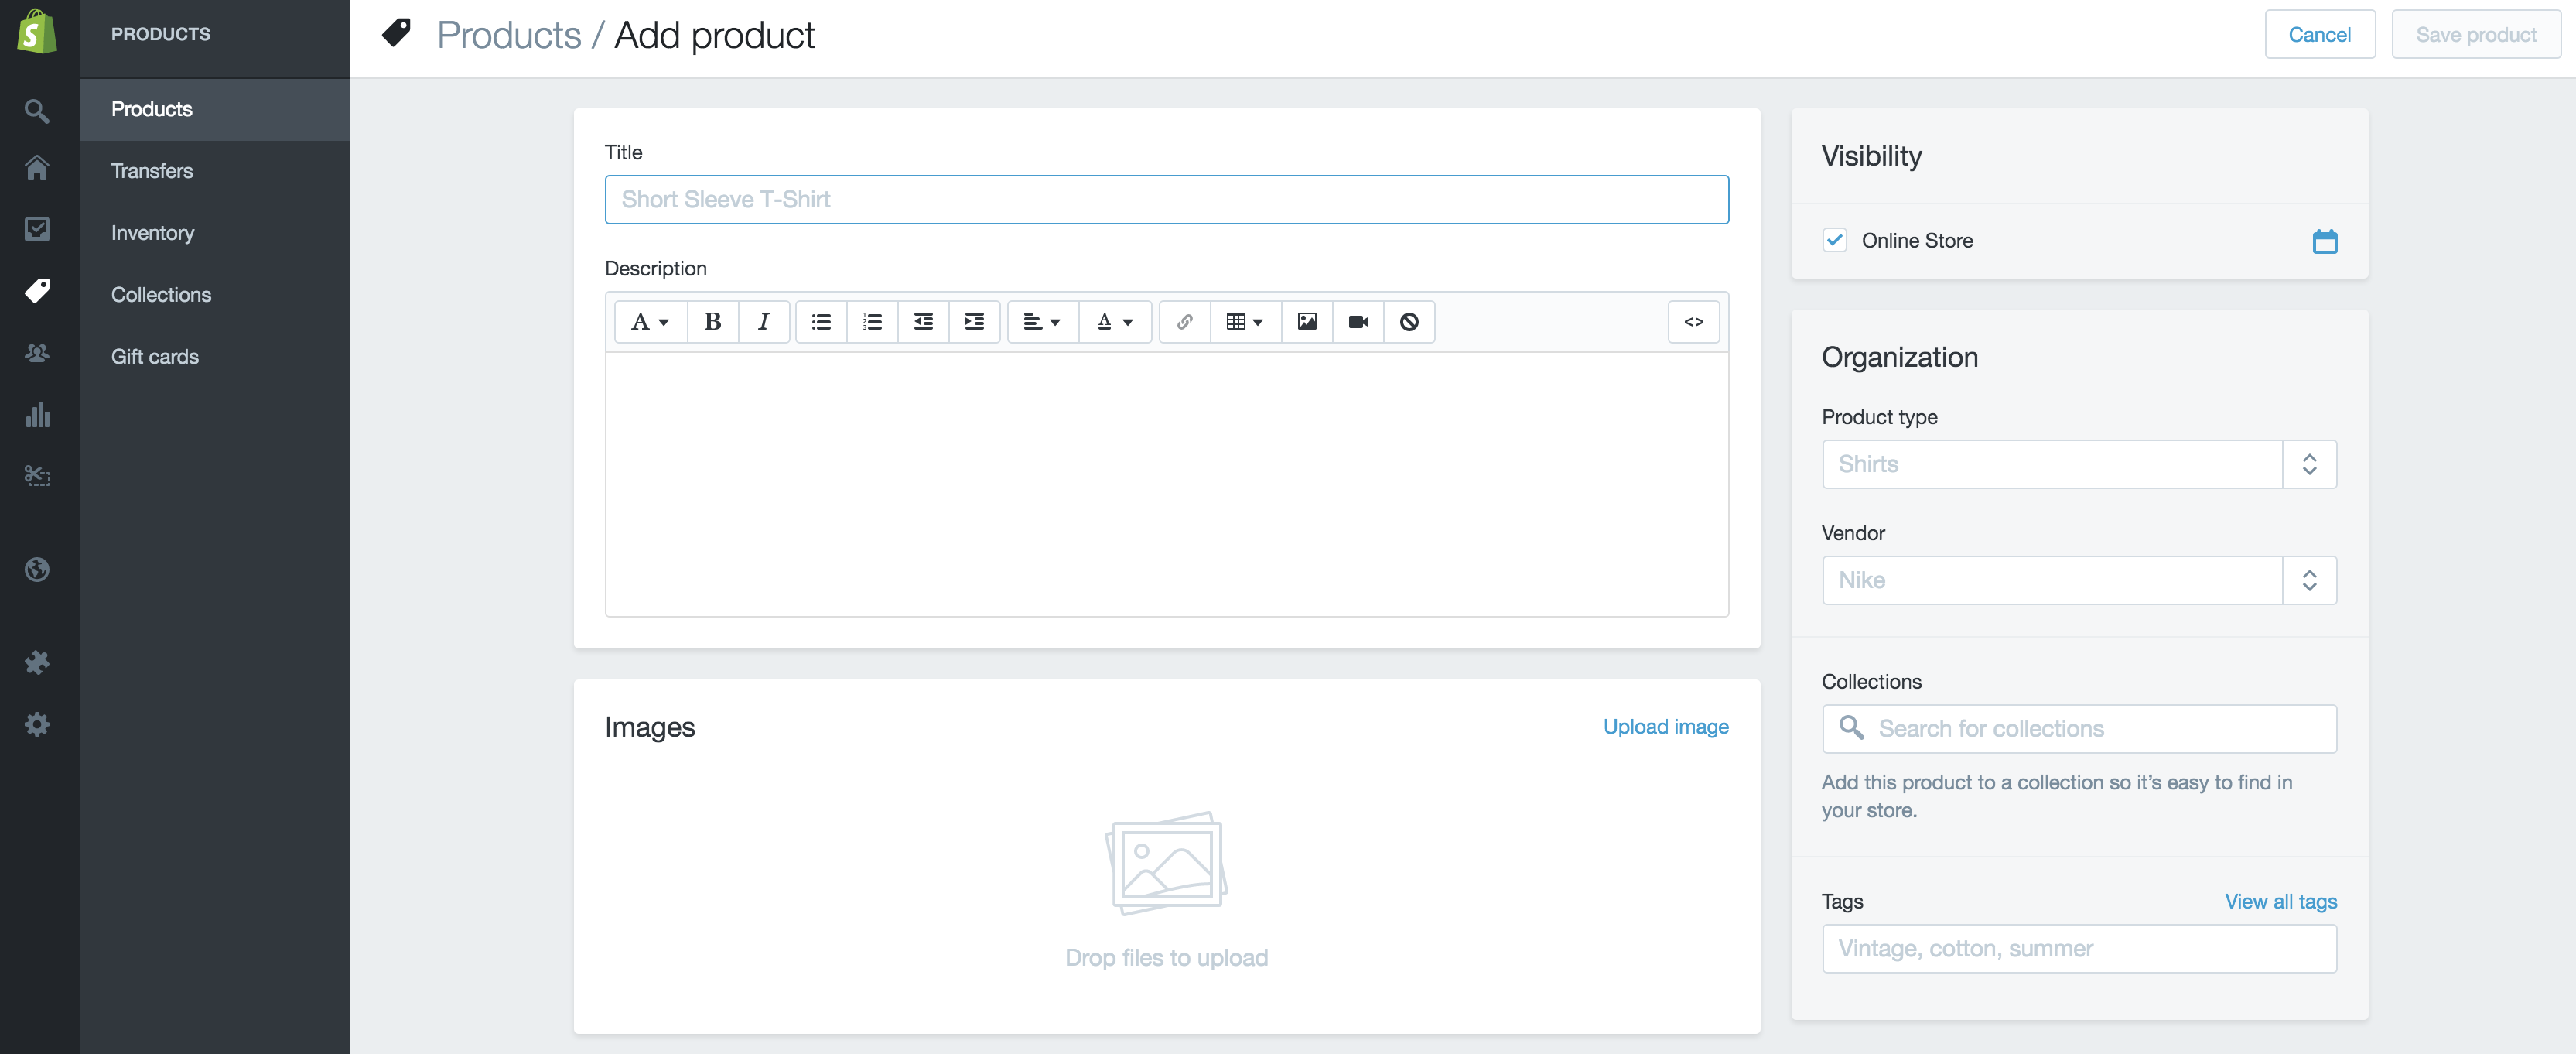
\includegraphics[width=1.0\linewidth]{images/chapter1/ex-shopify.png}\hfill
 \caption[Shopify Dashboard]{Shopify Dashboard}
 \label{fig:shopify_dashboard}
\end{figure}
\subsection{Bigcommerce}
Bigcommerce is a privately held technology company that develops e-commerce software for businesses. The company was founded in 2009 and has 370 employees with headquarters in Austin, Texas and additional offices in San Francisco, California and Sydney, Australia \cite{bigcommerce_overview}.
The company reports that \$5 billion in total sales have been processed by the Bigcommerce platform.
\begin{figure}[htb]
  \centering
  
\includegraphics[width=0.5\linewidth]{images/chapter1/bigcommerce_logo.jpg}\hfill
  \caption[Bigcommerce logo]{Bigcommerce logo}
  \label{fig:ebay_logo}
\end{figure}
Bigcommerce was founded in 2009 by Australians Eddie Machaalani and Mitchell Harper following a chance meeting in an online chatroom in 2003. In August 2009, the two relaunched a hosted version of Interspire Shopping Cart called “BigCommerce” and opened its first U.S. office.
\newline
Bigcommerce was 100\% bootstrapped until July 31, 2011, when it closed \$15 million in Series A funding from General Catalyst Partners. At the time, the company announced its client count had grown 680\% year over year. In January 2012, Bigcommerce launched a \$2 million integration fund for developers, which was used to fund 31 applications in the Bigcommerce App Marketplace. The company subsequently received \$20 million in Series B financing in September 2012, led by General Catalyst Partners and Floodgate Fund.
\subsection{Prestashop}
PrestaShop is a free, open source e-commerce solution and provides more than 250,000 online store owners with the most powerful, dynamic and international ecommerce software enriched with hundreds of innovative tools to build and manage a successful online store at no cost. PrestaShop is simple, efficient and intuitive with unmatched power that enables users to thrive in a competitive market regardless of size, industry or revenue \cite{prestashop_overview}.
\begin{figure}[htb]
  \centering
  
\includegraphics[width=0.5\linewidth]{images/chapter1/prestashop_logo.png}\hfill
  \caption[Prestashop logo]{Prestashop logo}
  \label{fig:ebay_logo}
\end{figure}
Used in over 200 countries and partnered with the most renowned names in the industry, PrestaShop continues to revolutionize online retail with technology that increases sales and maximizes visibility. Working hand in hand with its growing community of more than 850,000 dedicated members, PrestaShop’s entrepreneurial team is made up of ecommerce enthusiasts that are committed to the success and profitability of their online merchants.
PrestaShop started in 2005 as a student project within the EPITECH IT School in Paris, France. Originally named phpOpenStore, the software was first available in two languages: English and French. Three months after its launch the project was translated in thirteen languages.
\begin{figure}[htb]
 \centering
 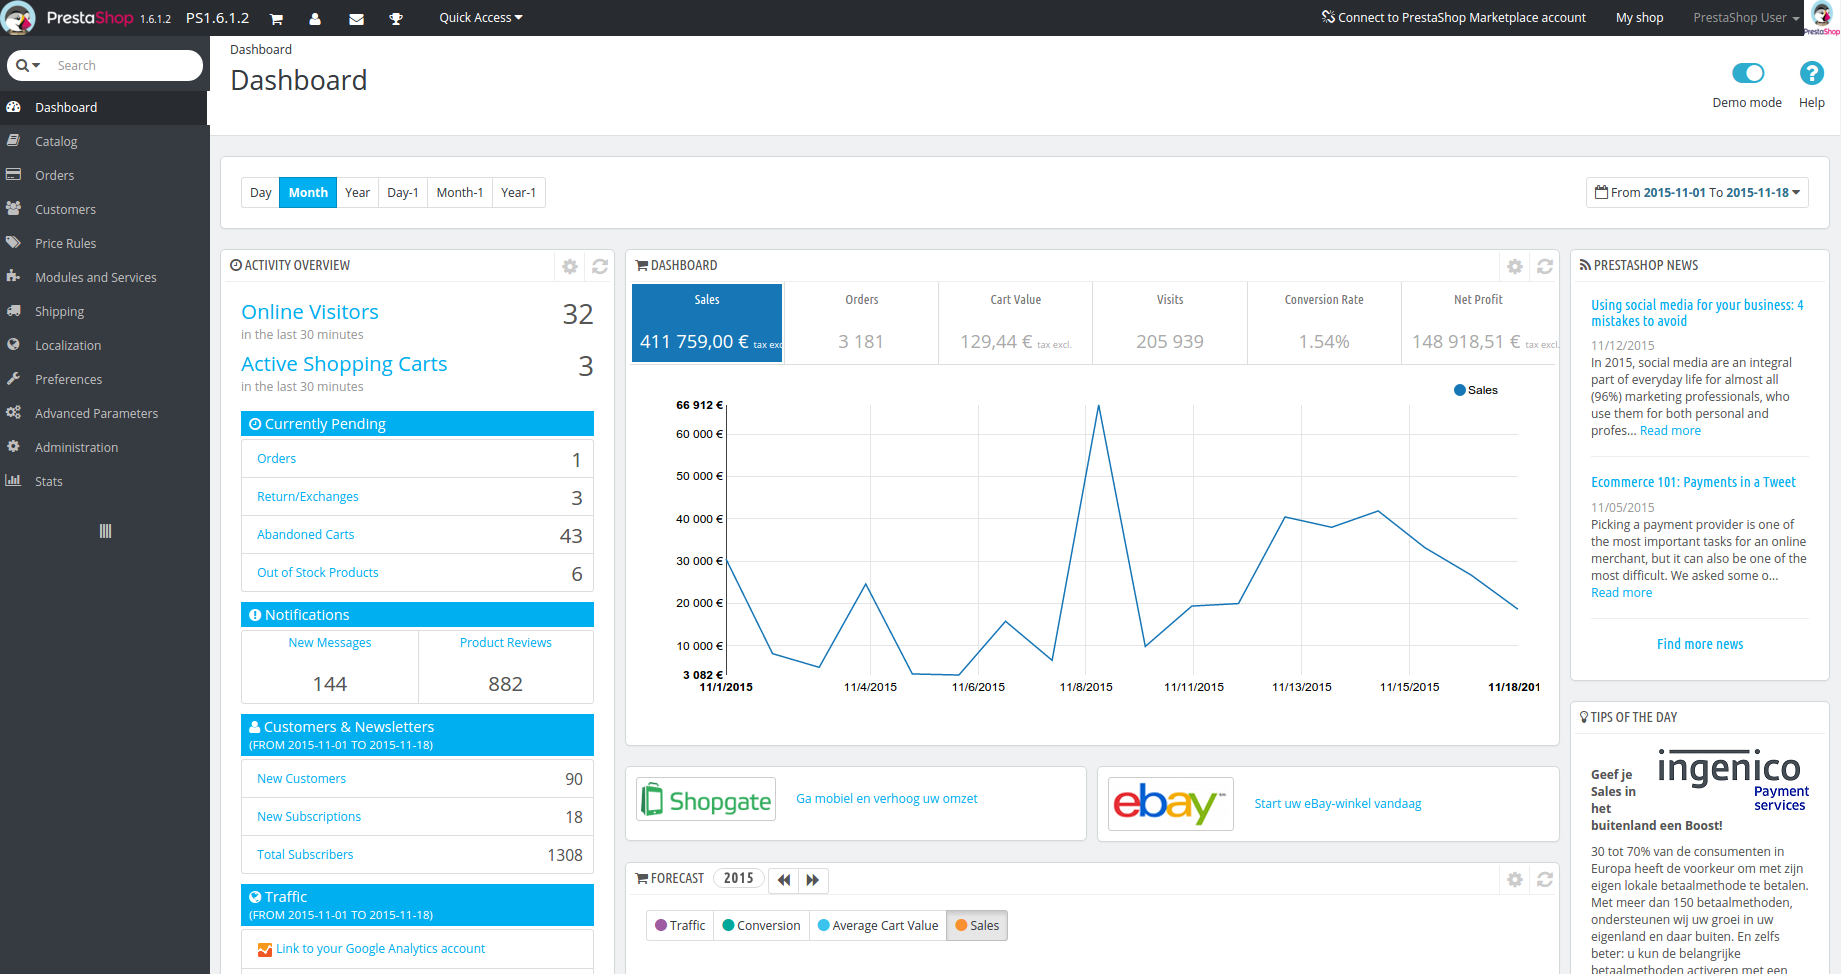
\includegraphics[width=1.0\linewidth]{images/chapter1/ex_prestashop.png}\hfill
 \caption[Prestashop Dashboard]{Prestashop Dashboard}
 \label{fig:prestashop_dashboard}
\end{figure}
The company, PrestaShop SA, was founded in 2007 by Igor Schlumberger and Bruno Lévêque. Between May 2010 and April 2012, PrestaShop grew from 17 employees to more than a hundred, with the establishment of secondary headquarters in Miami. In March 2014, PrestaShop SA secured \$9.3M in Series B Funding to continue its global expansion efforts. In January 2015, the company launched PrestaShop Cloud, a free self-hosted version of its software. According to technology tracking website BuiltWith.com, the market share of PrestaShop for open-source e-commerce websites is 9\%. According to W3Techs, PrestaShop is used by 0.5 of all websites \cite{prestashop_history}.


\chapter{Enabling services}
\label{cha:enabling_services}

This chapter describes enabling services.
\newline
A payment service provider (PSP) offers shops online services for accepting electronic payments by a variety of payment methods including credit card, bank-based payments such as direct debit, bank transfer, and real-time bank transfer based on online banking. Typically, they use a software as a service model and form a single payment gateway for their clients (merchants) to multiple payment methods \cite{payment_service_provider}.
\newline
The first section provides an overview of the Payment gatewayThe second and third sections describes the payment services focus Braintree and Stripe.
\newline
These services help the developer to integrate into their application payment systems easily. In particular, these services provide the libraries that are to be imported into your application to help manage the payment form. Each service provides a default form ready to be integrated in the application with a minimal interface(see \ref{sec:braintree} \ref{sec:stripe}).
\newline
The fourth section will discuss the issue of taxes that is very common problem for systems of e-commerce.

\section{Braintree}
\label{sec:braintree}
Braintree is a full-stack payments platform that makes it easy to accept payments in your app or website. Our service replaces the traditional model of sourcing a payment gateway and merchant account from different providers. From one touch payments to mobile SDKs and foreign currency acceptance, we provide everything you need to start accepting payments today.
\newline
All kinds of organizations use Braintree to accept payments in mobile apps and websites. From startups in garages, to not-for-profits, to some of the largest online retailers, we have more experience working with new business models than any other payments provider. However, due to legal and regulatory compliance reasons, Braintree isn't able to work with some business types. How to use Braintree as a payment system?
Braintree's  consists of complementary client and server SDKs:
\begin{itemize}
  \item The client SDK enables you to collect payment method (e.g. credit card, PayPal) details;
  \item The server SDKs manage all requests to the Braintree gateway
\end{itemize}
Before we get started, there are two key concepts to introduce - the client token and the payment method nonce.
\newline
SDK Braintree offer various options to the programmer to integrate the payment service.
\begin{figure}[htb]
  \centering
  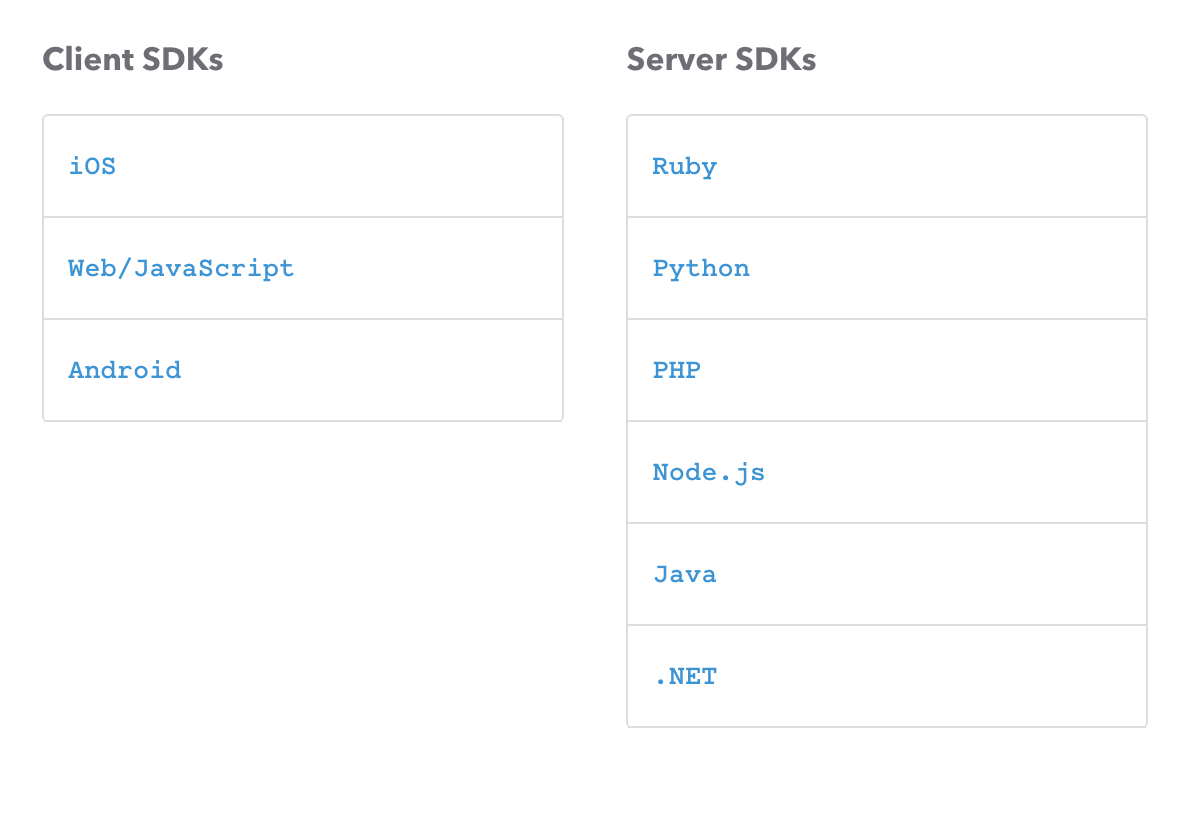
\includegraphics[width=1.0\linewidth]{images/chapter2/braintree-sdk.png}\hfill
  \caption[Braintree SDK]{Braintree SDK}
\label{fig:braintree_sdk}
\end{figure}
\subsection{Client Token}
A client token is a signed data blob that includes configuration and authorization information required by the Braintree Client SDK. These should not be reused; a new client token should be generated for each customer request that's sent to Braintree. For security, Braintree server revoke client tokens if they are reused excessively within a short time period.
The server is responsible for generating the client token, which contains all of the necessary configuration information to set up the client SDKs. When your server provides a client token to your client, it authenticates the application to communicate directly to Braintree.
The client is responsible for obtaining the client token and initializing the client SDK. If this succeeds, the client will generate a \emph{payment\_method\_nonce}.
\subsection{Payment Method Nonce}
The payment method nonce is a string returned by the client SDK to represent a payment method. This string is a reference to the customer payment method details that were provided in your payment form and should be sent to your server where it can be used with the server SDKs to create a new transaction request.
\begin{figure}[htb]
  \centering
  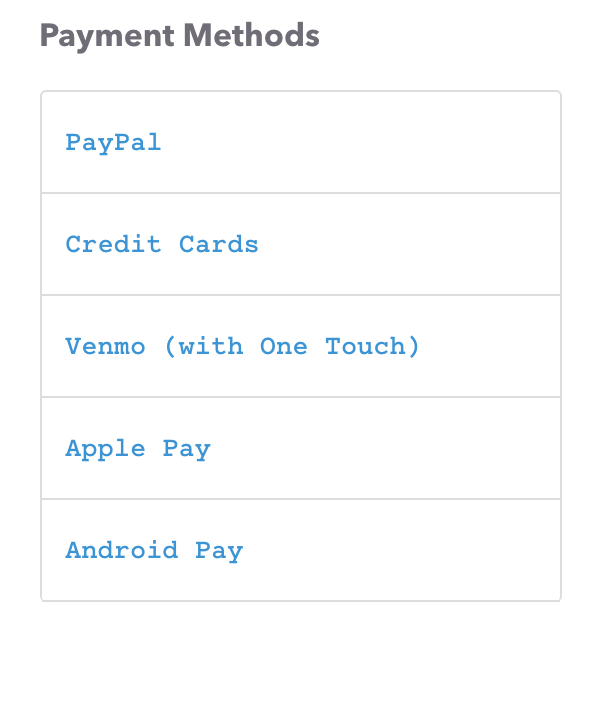
\includegraphics[width=0.4\linewidth]{images/chapter2/braintree-payment-method.png}\hfill
  \caption[Braintree payment method]{Braintree payment method}
  \label{fig:braintree_payment_method}
\end{figure}
Payment method nonces expire after 24 hours.
The server integration doesn't need to know the payment method type (e.g. credit card, PayPal account, Bitcoin) that is represented in the nonce. This means that your first v.zero integration should continue to work with few or no code changes when new payment method types are introduced.
\subsection{How it work}
\begin{figure}[htb]
  \centering
  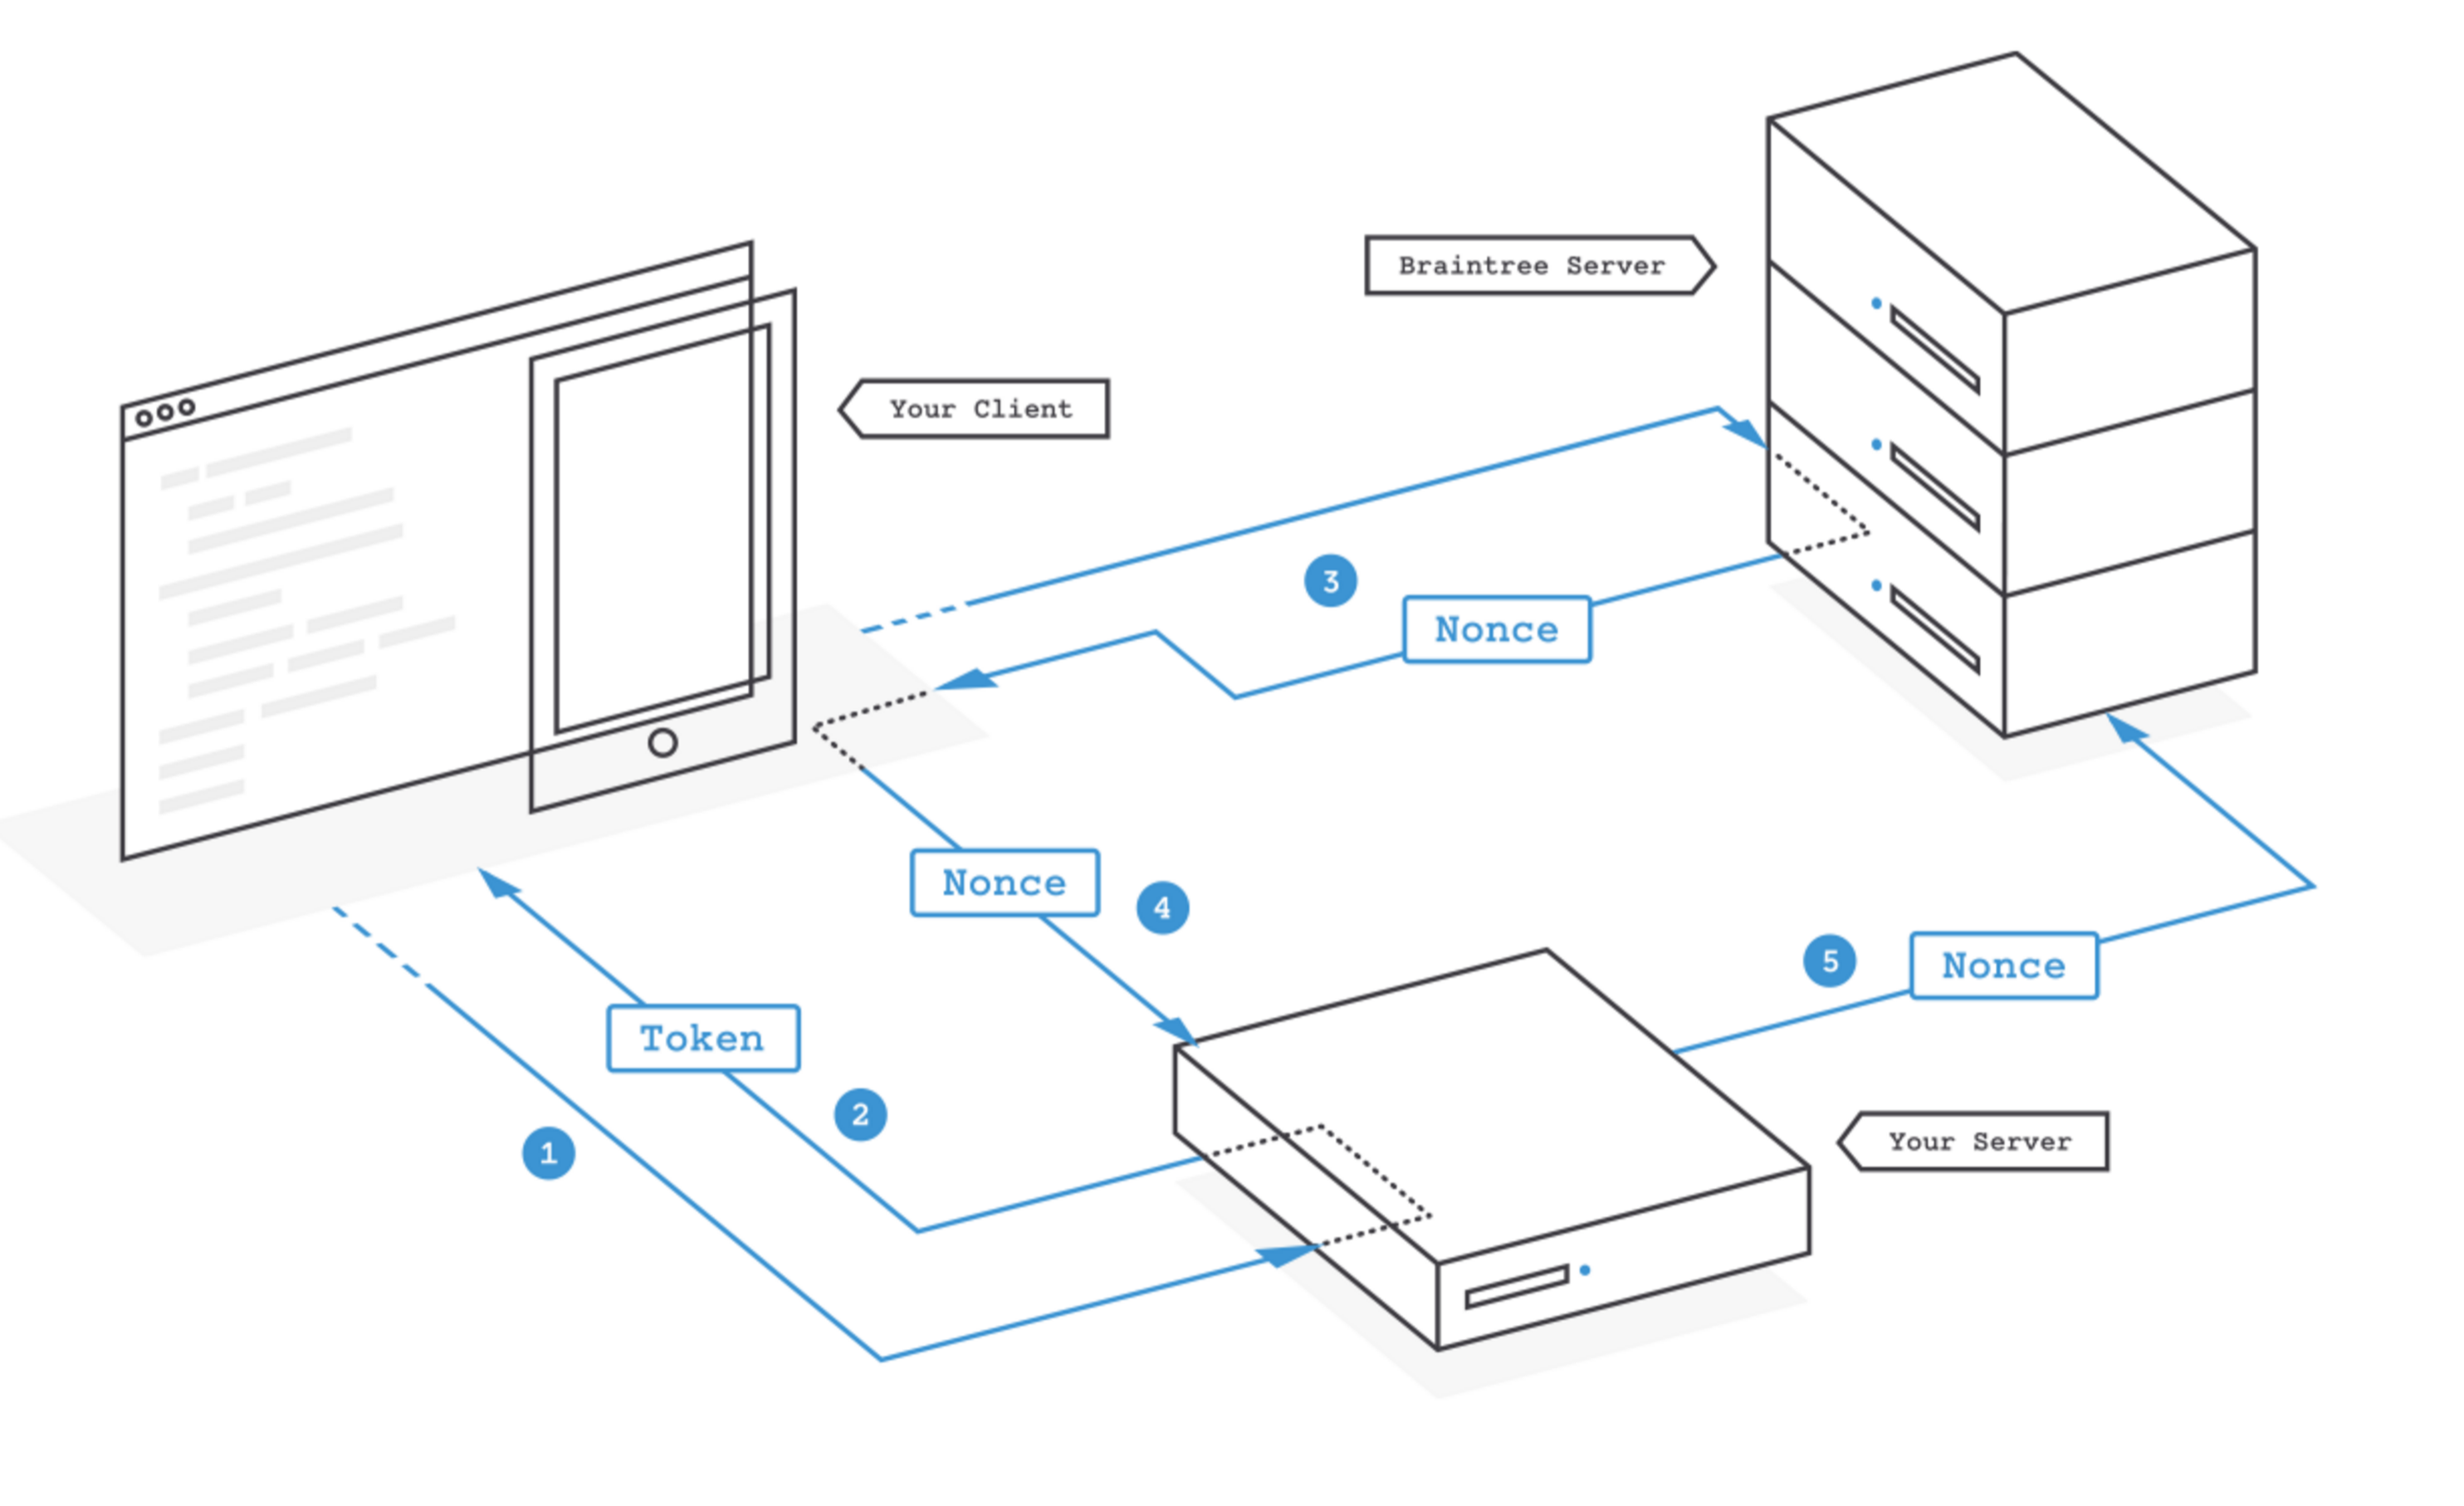
\includegraphics[width=1.0\linewidth]{images/chapter2/braintree-comunicaiton.png}\hfill
  \caption[Interaction client-braintree]{Comunication between client and server braintree step by step}
  \label{fig:braintree_server_comunication}
\end{figure}
\begin{enumerate}
  \item App or web front-end requests a client token from your server in order to initialize the client SDK;
  \item Server generates and sends a client token back to your client with the server SDK;
  \item Once the client SDK is initialized and the customer has submitted payment information, the SDK communicates that information to Braintree, which returns a payment method nonce;
  \item Then send the payment nonce to your server;
  \item Server code receives the payment method nonce from your client and then uses the server SDK to create a transaction or perform other Braintree functions.
\end{enumerate}
The easiest way to use braintree is through Drop-in UI. This type of configuration is certainly the simplest but allows the programmer to customize the input form for entering your payment information. The interface Drop-in looks like this as follows:
\begin{figure}[htb]
  \centering
  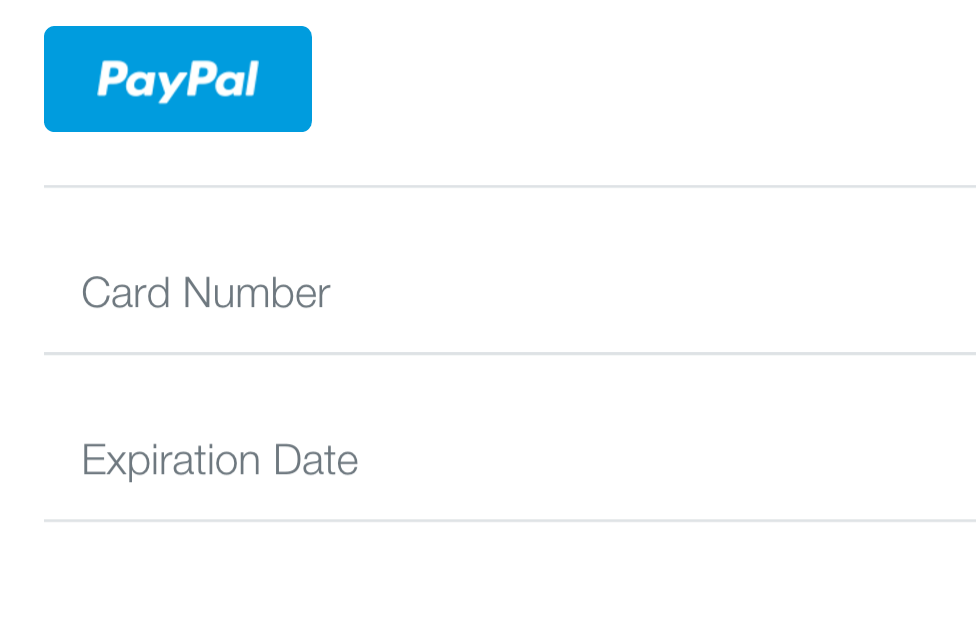
\includegraphics[width=0.6\linewidth]{images/chapter2/drop-in.png}\hfill
  \caption[Drop-in UI]{ Drop-in UI}
  \label{fig:drop_in_ui}
\end{figure}
To create and maintain this form to the client-side you must import the scrip \emph{brantree.js} and organize form so as follows:
\begin{lstlisting}[language=html]
<form id="checkout" method="post" action="/checkout">
  <div id="payment-form"></div>
  <input type="submit" value="Pay $10">
</form>

<script src="https://js.braintreegateway.com/v2/braintree.js"></script>
<script>
// We generated a client token for you so you can test out this code
// immediately. In a production-ready integration, you will need to
// generate a client token on your server.
var clientToken = client_token;

braintree.setup(clientToken, "dropin", {
  container: "payment-form"
});
</script>
\end{lstlisting}
To start up, braintree.js needs a client-token generated by your Braintree server SDK. The client-token is unique.
\newline
There are a number of ways to get your client token into JavaScript so you can set up Braintree. Many people choose to interpolate the client token into the HTML/JavaScript itself; alternatively, you could load the client token from an AJAX call to your exposed client token URL on your server.
Once you've finished this setup. Now we are ready to make payments.
\newline
A Braintree client-side integration sends payment information – like a credit card or a PayPal authorization – to Braintree in exchange for a payment method nonce, a one time use value that represents that payment method.
On your server, use a payment method nonce with a Braintree server SDK to charge a card or update a customers' payment methods.
\newline
By default, \emph{braintree.js} will add a hidden input named \emph{payment\_method\_nonce} to your form. When your user submits the form, if you have not subscribed to the \emph{onPaymentMethodReceived} callback, your form will be submitted with this value.
\newline
Braintree provides a sandbox for developers account, credit cards test for testing your application.
That said, we would like to use a form that is customizable to the way we would like to stylize the payment form without using the default. To do this simply specify additional parameters to the client side. How does this see in Chapter 5.

\section{Stripe}
\label{sec:stripe}
Stripe is the best way to accept payments online. Stripe aims to expand internet commerce by making it easy to process transactions and manage an online business.
\begin{figure}[htb]
\centering

\includegraphics[width=0.5\linewidth]{images/chapter2/stripe-logo.png}\hfill
\caption[Stripe logo]{Stripe logo}
\label{fig:stripe_logo}
\end{figure}
Stripe is 365 people and headquartered in an old trunk factory in the Mission district of San Francisco. The company has received around \$300 million in funding to date; investors include Sequoia Capital, Visa, American Express, Peter Thiel, and Elon Musk. Stripe enables you to accept payments in minutes. Collect your customers’ payment information easily and securely on web or mobile, and create charges server-side. Stripe supports 100+ currencies out of the box. In addition to credit and debit cards, Apple Pay, Android Pay, you can also easily support Bitcoin, Alipay, or Amex Express Checkout.
Stripe is a new widely celebrated alternative to Paypal and other payment gateways. Here are the main benefits of using the Stripe extension:
\begin{itemize}
\item Accept credit cards: process credit card orders directly on your site;
\item Increase sales: seamless checkout experience within your own site means increased conversions and/or sales;
\item Lower fees: competitive pricing (in many cases cheaper) than Paypal and other gateways;
\item Advanced analytics \& reporting – Beautiful analytics dashboard and sales reporting in Stipe.com;
\item PCI compliance: keeps your customers’ data safe on Stripe’s PCI compliant servers;
\item Incredibly simply setup and configuration. Buyers never leave your site to make the purchase;
\item No hidden fees: don’t get charged for refunds or disputes;
\item Global: business in any of these countries can accept payments from customers anywhere in the world;
\end{itemize}
\subsection{How it works}
Even Stripe, as Braintree, provides a default widget that you can use to integrate payments.
\begin{figure}[htb]
  \centering
  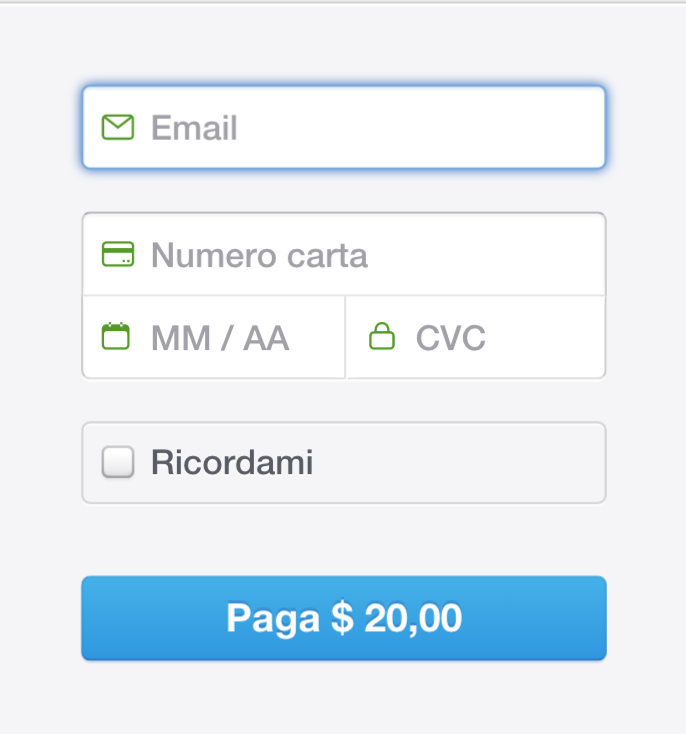
\includegraphics[width=0.5\linewidth]{images/chapter2/stripe-drop.png}\hfill
  \caption[Default stripe payment widget]{Default stripe payment widget}
\label{fig:stripe_default_ui}
\end{figure}
To get this widget, just enter the following code in its page:
\begin{lstlisting}[language=html]
<form action="" method="POST">
  <script
    src="https://checkout.stripe.com/checkout.js" class="stripe-button"
    data-key="pk_test_6pRNASCoBOKtIshFeQd4XMUh"
    data-amount="2000"
    data-name="Demo Site"
    data-description="2 widgets ($20.00)"
    data-image="/128x128.png"
    data-locale="auto">
  </script>
</form>
\end{lstlisting}
The most important thing to notice is the data-key attribute added to the script tag. This key identifies your account when communicating with Stripe.
\newline
Stripe also offers the ability to customize the payment form. This and other details can be discussed in Chapter 5.

\section{Polymer}
\label{sec:polymer}
This section there will be an overview of Polymer. Polymer provides a thin layer of API on top of Web Components and several powerful features, such as custom events and delegation, mixins, accessors and component life- cycle functions, to facilitate the creation of Web Components. Polymer does this by:
\begin{itemize}
\item Allowing to create Custom Elements with user-defined naming schemes. These custom elements can then be distributed across the network and used by others with HTML Imports
\item Allowing each custom element to have its own template accompanied by  styles and behavior required to use that element
\item Providing a suite of ready-made UI and non-UI elements to be used and extended in projects
\item The elements collection of Polymer is divided into more  sections:
\item Core Elements — These are a set of visual and non-visual elements designed to work with the layout, user interaction, selection, and scaf- folding applications.
\item Paper Elements — Implement the material design philosophy launched by Google recently at Google I/O 2014, and these include everything from a simple button to a dialog box with neat visual effects.
\item Iron Elements — A set of visual and non-visual utility elements. It includes elements for working with layout, user input, selection, and scaffolding apps.
\item Gold Elements — The gold elements are built for e-commerce use-cases like checkout flows.
\item Neon Elements — Neon elements implement special effects.
\item Platinum Elements — Elements to turn web pages into a true webapp, with push, offline, and  more.
\item Molecules — Molecules are elements that wrap other javascript li- braries.
\end{itemize}
\begin{figure}[htb]
 \centering
 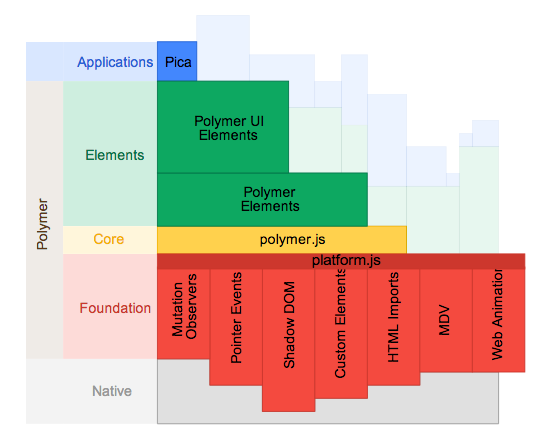
\includegraphics[width=1.0\linewidth]{images/chapter2/polymer-architecture.png}\hfill
 \caption[Polymer Architecture]{Polymer Architecture}
 \label{fig:fourV}
\end{figure}
Web components standards provide the needed primitives to build new components. It is possible to build custom elements using these primitives, but it can be a lot of work.
\newline
The Polymer library provides a declarative syntax that makes it simpler to define custom elements. Furthermore, it adds features like templating, two-way data binding and property observation to help developers build powerful, reusable elements with less code.
\newline
Custom elements. If users don’t want to write their own elements, there are a number of elements built with Polymer that it is possible to drop straight into existing pages. These elements depend on the Polymer library, but they can be used without using Polymer directly, as well.[6]
\newline
Polymer is one of the first implementations of a user interface library  built upon the Web Components standard. Web Components are not fully supported by browsers, but they provide a polyfill library, webcomponents.js, that provides enough functionality to support Web Components and Polymer.
\newline
Web Components standard is the result of the evolution of user interface libraries over the past decade, finally reaching the goal of separating HTML, CSS and JavaScript and running HTML through W3C validators. For exam- ple, looking at a .css file, it is possbile to easily determine which selectors are actually used in HTML and especially programmatically used in JavaScript. Similarly, it is easy to organize JavaScript code so that everything could be reused efficiently on multiple pages.[23]

\section{Easypost}
\label{sec:easypost}
Another key point in the systems of e-commerce is the delivery and tracking of parcels. From the logistics point of view this is a very complicated problem to which we must pay close attention today because customer satisfaction is strongly dependent on the traceability of its services well. Through this feature the customer is aware of when you receive the order.
\begin{figure}[htb]
  \centering
  
\includegraphics[width=0.5\linewidth]{images/chapter2/shipment-tracking.jpg}\hfill
  \caption[shipping and tracking]{shipping and tracking}
\label{fig:shipping_tracking}
\end{figure}
Easypost is a service that solves problems related notes to shipments and tracking of packages offering a solution well established. Following is an example in code to send a parcel:
\begin{lstlisting}[language=javascript]
var easypost = require('node-easypost')(apiKey);
// set addresses
var toAddress = {
  name: "Dr. Steve Brule",
  street1: "179 N Harbor Dr",
  city: "Redondo Beach",
  state: "CA",
  zip: "90277",
  country: "US",
  phone: "310-808-5243"
};
var fromAddress = {
  name: "EasyPost",
  street1: "118 2nd Street",
  street2: "4th Floor",
  city: "San Francisco",
  state: "CA",
  zip: "94105",
  phone: "415-123-4567"
};

// verify address
easypost.Address.create(fromAddress, function(err, fromAddress) {
  fromAddress.verify(function(err, response) {
    if (err) {
      console.log('Address is invalid.');
    } else if (response.message !== undefined && response.message !== null) {
      var verifiedAddress = response.address;
    } else {
      var verifiedAddress = response;
    }
  });
});

// set parcel
easypost.Parcel.create({
  predefined_package: "InvalidPackageName",
  weight: 21.2
}, function(err, response) {
  console.log(err);
});

var parcel = {
  length: 10.2,
  width: 7.8,
  height: 4.3,
  weight: 21.2
};

// create customs_info form for intl shipping
var customsItem = {
  description: "EasyPost t-shirts",
  hs_tariff_number: 123456,
  origin_country: "US",
  quantity: 2,
  value: 96.27,
  weight: 21.1
};

var customsInfo = {
  customs_certify: 1,
  customs_signer: "Hector Hammerfall",
  contents_type: "gift",
  contents_explanation: "",
  eel_pfc: "NOEEI 30.37(a)",
  non_delivery_option: "return",
  restriction_type: "none",
  restriction_comments: "",
  customs_items: [customsItem]
};
// create shipment
easypost.Shipment.create({
  to_address: toAddress,
  from_address: fromAddress,
  parcel: parcel,
  customs_info: customsInfo
}, function(err, shipment) {
  // buy postage label with one of the rate objects
  shipment.buy({rate: shipment.lowestRate(['USPS', 'ups']), insurance: 100.00}, function(err, shipment) {
    console.log(shipment.tracking_code);
    console.log(shipment.postage_label.label_url);
  });
});
\end{lstlisting}


\chapter{Enabling services}
\label{cha:enabling_services}

This chapter describes X-commerce enabling technologies.
The first section provides an overview of Single Page Application development pattern.
The second,third and fourth sections concern server-side technologies: MongoDB, NodeJS and Loopback by Strongloop (an IBM company). MongoDB is a NoSQL document-oriented database management system; NodeJS is an event-driven framework to handle Javascript server sides; Loopback is a NodeJS based framework created to use and edit set of APIs.
The fifth, sixth and seventh sections are related to client-side technologies: HTML5, Web Components and Polymer-Project by Google. HTML5 is a markup language aimed at web pages structuring; Web Components are a set of standards that allow for the creation of reusable widget and components in  web  documents;  Polymer-Project provides a thin layer  of API on top of Web Components and several powerful features, such as custom events, delegation, mixins, accessors and component life-cycle functions, to facilitate the creation of Web  Components.

\section{x-commerce overview}
\label{sec:x_commerce_overview}
X-commerce is a web platform for building e-commerce systems. This platform build full-stack Javascript NodeJS API-centric HTML5 based Single Page Application with Web Components via Polymer- Project.  In particular, the core of x-commerce follows the philosophy of Polymer project or all the complex parts of the platform are self-contained and isolated so that responsibilities are well localized. In other words, x-commerce has been developed to facilitate the modifiability of the code, integrity of new services and reusability. This is facilitated thanks to Polymer for which: “Everything is an element, even a service”.
So, a Web plathform is essentially built by composing elements together.
\newline
For example a page of a product has been divided into various element and each element contributes to realize the same page. In this way any changes related to the code are very well located. In following it is a more abstract level is designed as a page in general.
\begin{figure}[htb]
 \centering
 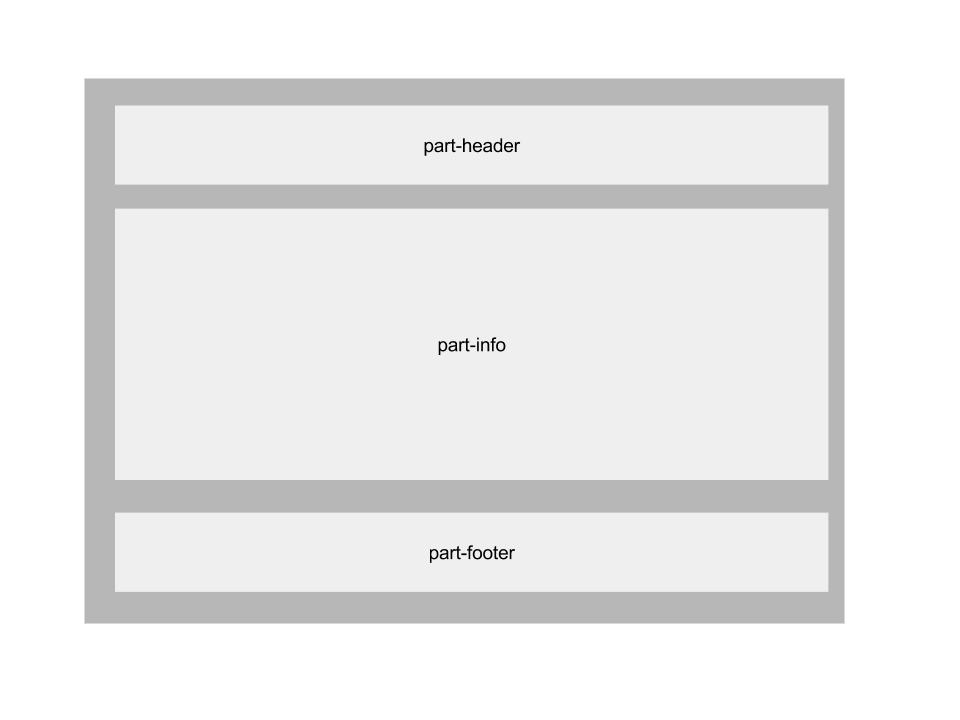
\includegraphics[width=1.0\linewidth]{images/chapter3/design-page.jpg}\hfill
 \caption[Design page]{Example of how the pages are designed}
 \label{fig:design_page}
\end{figure}
So e-commerce is a platform developed for compositions of elements. This philosophy also helps code reusability. In fact, in the navigation of web pages, between the previous and the next, there is a lot in common such as header and footer. With web components, so, they also create elements that are often used by most parties.
Moreover, thanks to Web Components philosophy and X-Project guidelines, it’s easy to gain a clear separation between structure, content, behavior and presentation of elements. It’s possible to create components that concern the only presentation part of an element, such as mixins in which developers can express groups of CSS rules to be applied to different elements.
\newline
On a small project, the potential of Polymer may not be very obvious, but when the project is large the philosophy that “everything is an element” helps a lot in design and construction.
\newline
We see in the following paragraphs as the complexity of x-commerce was demolished by creating elements.

\section{HTML5}
\label{sec:html5}
This section provides an overview of HTML5.
HTML5 is the latest version of Hypertext Markup Language, the code
\begin{figure}[htb]
 \centering
 
\includegraphics[width=1.0\linewidth]{images/chapter3/tecnologie.jpeg}\hfill
 \caption[Server and client sides enabling  technologies]{Server and client sides enabling  technologies}
 \label{fig:fourV}
\end{figure}
that describes web pages. There are actually three kinds of code: HTML, which provides the structure; Cascading Style Sheets (CSS), which take care of presentation; and JavaScript, which makes things happen.
\newline
HTML5 has been designed to deliver almost everything it is possible to do online without requiring additional software such as browser plugins. It does everything, from animation to apps, music to movies, and can also be used to build complicated applications that run in browsers.
\newline
Moreover, HTML5 isn’t proprietary, so it is completely free. It’s also a cross-platform standard, which means it doesn’t care whether the device is a tablet or a smartphone, a netbook, notebook or ultrabook or a Smart TV: if the browser supports HTML5, it should work  flawlessly.
\newline
While some features of HTML5 are often compared to Adobe Flash, the two technologies are very different. Both include features for playing audio and video within web pages, and for using Scalable Vector Graphics. HTML5, on its own, cannot be used for animation or interactivity, it must be supplemented with CSS3 or JavaScript. There are many Flash capabilities  that have no direct counterpart in HTML5. See Comparison of HTML5 and Flash.
\begin{figure}[htb]
 \centering
 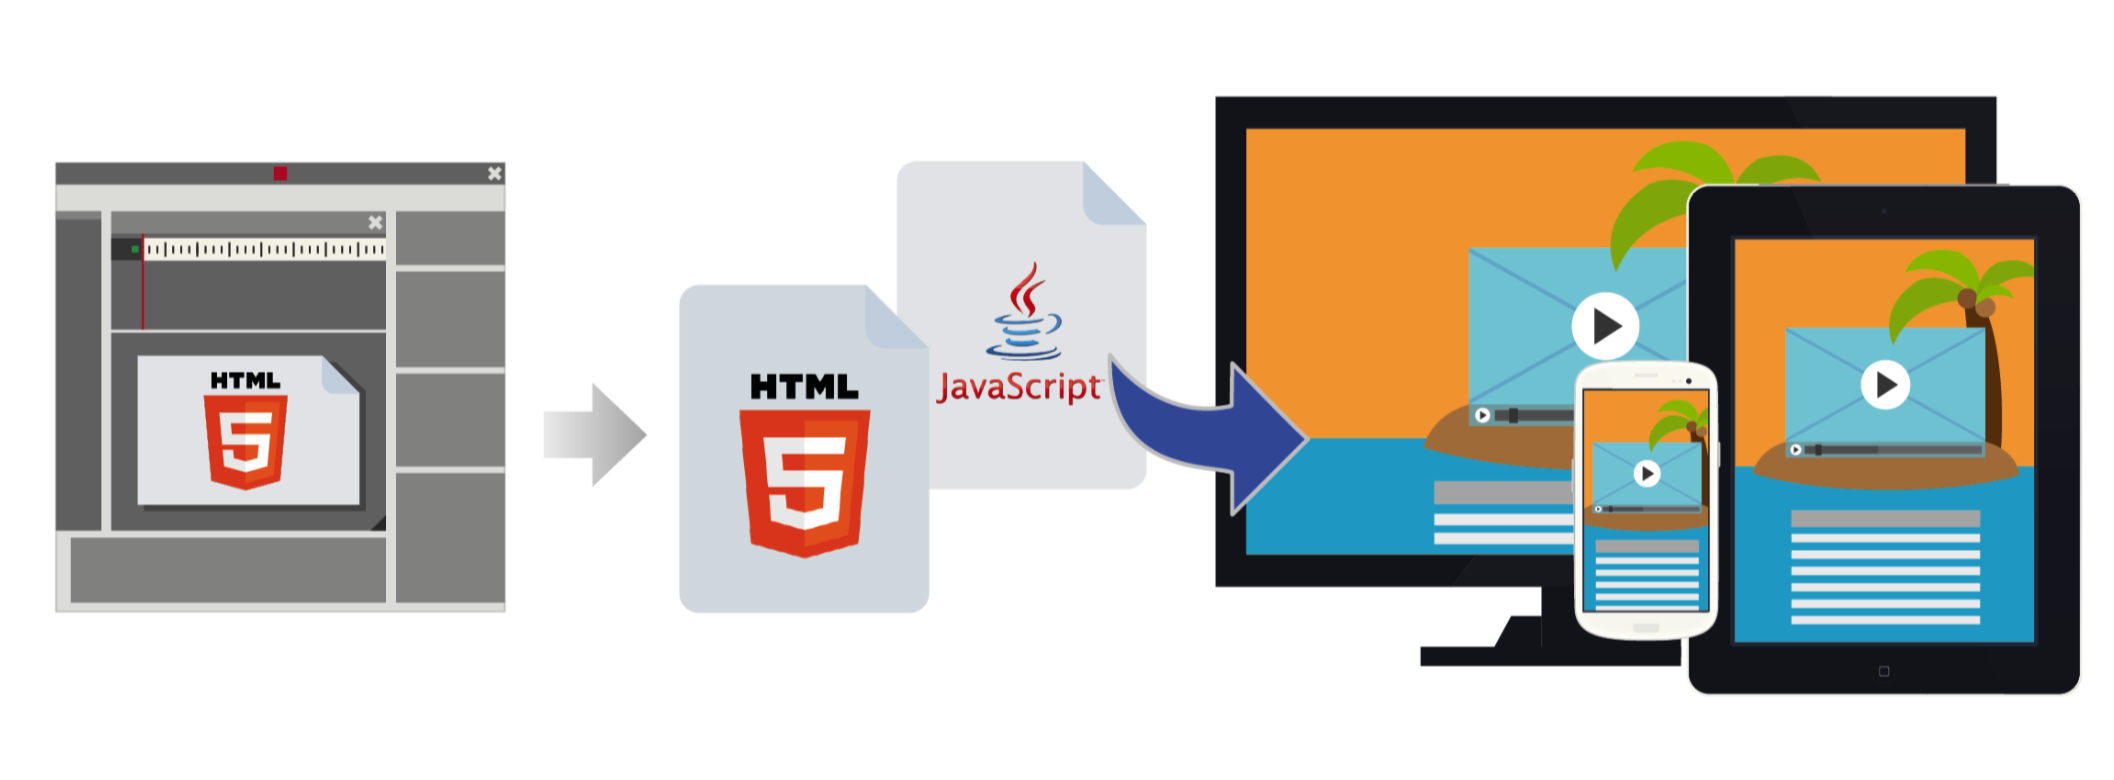
\includegraphics[width=1.0\linewidth]{images/chapter3/Html5_responsive.png}\hfill
 \caption[Html5 Responsive]{Html5 Responsive}
 \label{fig:fourV}
\end{figure}
Although HTML5 has been well known among web developers for years, its interactive capabilities became a topic of mainstream media around April 2010, after Apple Inc’s then-CEO Steve Jobs issued a public letter entitled “Thoughts on Flash”  where he concluded that “Flash is no longer necessary to watch video or consume any kind of web content” and that “new open standards created in the mobile era, such as HTML5, will win”.This sparked a debate in web development circles where some suggested that while HTML5 provides enhanced functionality, developers must consider the varying browser support of the different parts of the standard as well as other functionality differences between HTML5 and Flash. In early November 2011, Adobe announced that it would discontinue development of Flash for mobile devices and reorient its efforts in developing tools using HTML5.


In conclusions...



\part{Part 2}
\label{part:part_2}


\chapter{Enabling services}
\label{cha:enabling_services}

This chapter presents the core of the thesis project: X-commerce.
The first section provides a project’s overview, giving reasons of development, listing benefits and functions. The second section describe Single Page Application development pattern. The third section shows the x-commerce architectural stack and the reasons why these technologies have been chosen. The fourth section presents the development methodology that has been thought for the project. In the fifth paragraph shows the models and their APIs basic x-commerce.

\section{x-commerce overview}
\label{sec:x_commerce_overview}
X-commerce is a web platform for building e-commerce systems. This platform build full-stack Javascript NodeJS API-centric HTML5 based Single Page Application with Web Components via Polymer-Project. In particular, the core of x-commerce follows the philosophy of Polymer project or all the complex parts of the platform are self-contained and isolated so that the responsibilities are well localized. In other words, x-commerce has been developed to facilitate the modifiability of the code, integrity of new services and reusability. This is facilitated, thanks to Polymer for which: “Everything is an element, even a service.”
So, a Web platform is essentially built by composing elements together.
\newline
For example a page of a product has been divided into various elements and each element contributes to realize the same page. In this way any changes related to the code are very well located. In following it is, a more abstract level designed as a page in general.
\newpage
\begin{figure}[htb]
 \centering
 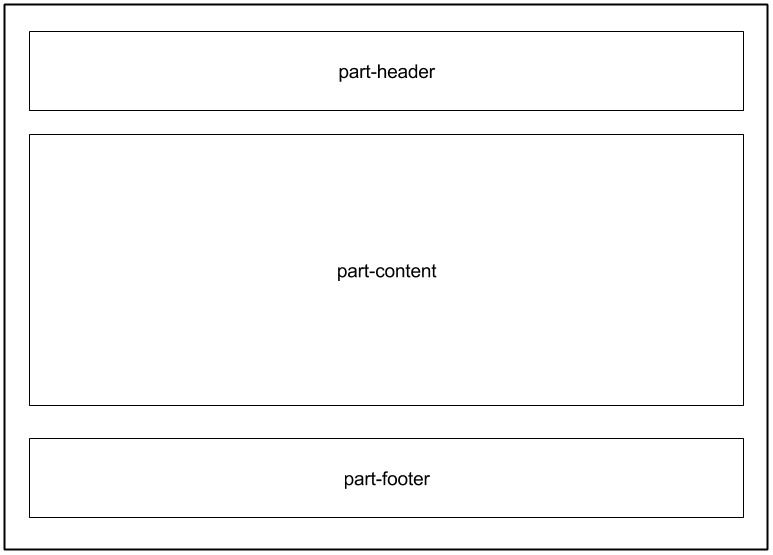
\includegraphics[width=1.0\linewidth]{images/chapter4/design-page.png}\hfill
 \caption[Design page]{Example of how the pages are designed}
 \label{fig:design_page}
\end{figure}
So e-commerce is a platform developed for composition of elements. This philosophy also aids code reusability. In fact, in the navigation of web pages, between the previous and the next, there is a lot in common, such as header and footer. With the Web components, the elements that are often used by most parties are also created.
Moreover, with help of the Web Components philosophy, it’s easy to gain a clear separation between structure, content, behavior and presentation of elements. It is possible to create components that are related only to the presentation part of an element, such as mixins in which developers can express groups of CSS rules to be applied to different elements.
\newline
On a small project, the potential of Polymer may not be very obvious, but when the project is large the philosophy that “everything is an element” helps a lot in design and construction.

\section{Single Page application}
\label{sec:signle_page_application}
Single-page application (SPA) is a web application or web site that fits on a single web page with the goal of providing a more fluid user experience akin to a desktop application. In a SPA, either all necessary code – HTML, JavaScript, and CSS – is retrieved with a single page load,[31] or the appropriate resources are dynamically loaded and added to the page as necessary, usually in response to user actions. The page does not reload at any point in the process, nor does control transfer to another page, although modern web technologies (such as those included in the HTML5 pushState() API) can provide the perception and navigability of separate logical pages in the application. Interaction with the single page application often involves dynamic communication with the web server behind the scenes.
\newline
SPAs use AJAX and HTML5 to create fluid and responsive Web apps, without constant page reloads. However, this means much of the work hap- pens on the client side, in JavaScript. For the traditional ASP.NET developer, it can be difficult to make the leap. Luckily, there are many open source JavaScript frameworks that make it easier to create SPAs.
In a traditional Web app, every time the app calls the server, the server renders a new HTML page. This triggers a page refresh in the browser.
\begin{figure}[htb]
 \centering
 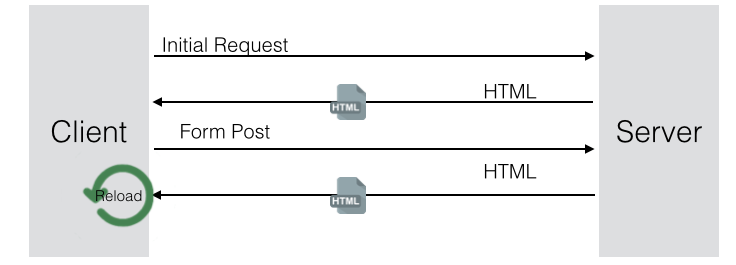
\includegraphics[width=1.0\linewidth]{images/chapter4/trad_life.png}\hfill
 \caption[Traditional Page Lifecycle]{The Traditional Page Lifecycle}
 \label{fig:traditional_page_lifecycle}
\end{figure}
In an SPA, after the first page loads, all interaction with the server happens through AJAX calls. These AJAX calls return data - not markup - usually in JSON format. The app uses the JSON data to update the page dynamically, without reloading the page.
One benefit of SPAs is obvious: Applications are more fluid and responsive, without the jarring effect of reloading and re-rendering the page.
\begin{figure}[htb]
 \centering
 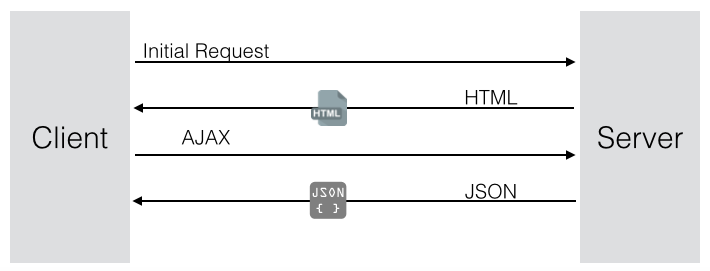
\includegraphics[width=1.0\linewidth]{images/chapter4/spa_life.png}\hfill
 \caption[SPA Lifecycle]{The SPA Lifecycle}
 \label{fig:spa_lifecycle}
\end{figure}

\section{x-commerce design}
\label{sec:document_driven_web_development_process}
At the design stage, we have identified two solutions for the management of the resources used by the client and by the administrator of x-commerce. In particular, the client of x-commerce have different needs in the use of the platform than the administrator. While the former is more oriented to the use of the information on products and eventually to the order, the administrator is more concerned with the inclusion of new products and information in order to better organize the resources and the interface offered to the customer. Considering that the two main actors involved in these interactions require different levels of security. Only the administrator can modify the information and all other eligible data.
\newline
To separate this client management and administrator e-commerce, it was decided to separate the pages of the administrator and client in two different directories. This allows you to host the administrator on a server other than the server on which the client access to x-commerce. This does not however exclude the possibility of offering two types of services from a single server.
\newline
This organization of pages for the client and the administrator allows you to assign the same name to the pages and its parts.
\newline
The process to build a web application based on x-commerce toolkit consists of the following four steps: defining the model of the schema, HTTP RESTful API definition, UI components definition and assembly.
\subsection{Model schemas definition}
A description of entities, properties, relations and data access policies are defined as JSON documents.
\newline
The models of e-commerce are many and are expected to grow further with the integration and implementation of new services. At the moment there are 30 models. Loopback in the definition of each model is done by filling in a JSON file where declare properties that interest us. In the following are the main models of x-commerce:
\begin{itemize}
\item \emph{product}: the model has many properties, but we are specifying the properties which are of greater interest; for which:
\begin{itemize}
\item a product has a title string (we are also saying that this field is required);
\item a product has a description string;
\item a product has a price of type Number, etc..
\end{itemize}
The model has also produced the “relations”. This field identifies relation of the current model (“product”) with other models such as:
\begin{itemize}
\item a product has a relationship with the model “Image” type “many”. This report was modeled because the product has a lot of pictures;
\item a product has the relationship with the model “Comments” type “many” because a product has many comments or reviews, etc.
\item it is possible also to specify “acls (access control lists)” to control access to the system. Thus by specifying who can do what with a JSON file, it is possible to have a transparent way all security mechanisms.
\end{itemize}
\begin{lstlisting}[language=json]
{
  "name": "Product",
  "properties": {
    "title": { "type": "String", "required": true },
    "description": { "type": "String" },
    "price":  { "type": "Number" },
  },
  "relations": {
    "images": { "type": "hasMany", "model": "Image" },
    "comments": { "type": "hasMany", "model": "Comment" },
    "collections": { "type": "hasAndBelongsToMany", "model": "Collection" },
    "options": { "type": "hasMany", "model": "ProductOption" },
    "product_type": { "type": "belongsTo", "model": "ProductType" },
    "variants": { "type": "hasMany", "model": "ProductVariant" },
    "vendor": { "type": "belongsTo", "model": "Vendor"}
  }
}
\end{lstlisting}
\item \emph{customers}: this time there are two new things:
\begin{itemize}
\item the presence of \emph{acls}: in this case acls block all calls except “find” and count” that can call all;
\item note the presence of the \emph{“base”: “Users”}: “Users” is a model of loopback that is offered for free. This model brings back all funtionality related to login, sign up, forgot etc. “Customer” model extends the “Users” loopback, and in this way the “Customer” legacy capabilities and therefore all methods APIs and “Users” including methods for login and logout.
\begin{lstlisting}[language=json]
{
  "name": "Customer",
  "base": "User",
  "properties": {
    "first_name": { "type": "String", "required": true },
    "last_name": { "type": "String", "required": true },
    "date_of_birth" : { "type": "Date" },
    "gender": { "type": "String", "enum": ["M", "F"] },
    "email": { "type": "String", "required": true }
  }
}
\end{lstlisting}
\end{itemize}
\end{itemize}

Each JSON file is also accompanied by a js file. This file is used to define the so-called “hooks” or the methods to define new APIs customized. These new APIs are added to the API generated by the JSON file.
\begin{lstlisting}[language=javascript]
module.exports = function (Product) {
};
\end{lstlisting}
Inside the function offered to extend the API, it is possbile to define new APIs. The name of the API is declared as follows:
\begin{lstlisting}[language=javascript]
module.exports = function (Product) {
  Product.remoteMethod('generate_variants', {
    accepts: { arg: 'product_id', type: 'string', required: true },
    returns: { arg: 'variants', type: 'Array' },
    http: { verb: 'get', path:'/generate”' }
  });
};
\end{lstlisting}
The remote method takes two parameters:
\begin{itemize}
\item the name of the method to execute the call of the API in question. In this way, the method name is “generate\_variants”. This method will be executed when it is called api: “/api/Products/generate”;
\item as the second parameter, the remote method accepts a JSON object consisting of key-value pairs:
\begin{itemize}
\item “accepts”: indicates the input parameters that is, parameters that are present in the body of the request. In this case the input parameter is the only one and is of type String and is required.
\item “returns”: It indicates what type is the response;
\item “http”: This is a parameter that defines url API. Therefore, url for calling the generate API is: “/api/Products/generate”. When you call this API, it is invoked and executed the remote method declared as the first parameter. The remote method must be defined freely by the programmer.
\end{itemize}
\end{itemize}
Therefore, the complete example to define new APIs via remote methods, which are not generated by default from JSON file, is the following:
\begin{lstlisting}[language=javascript]
module.exports = function (Product) {
  Product.generate_variants = function (product_id, callback) {
    // to do anythings. Genreate a result
    callback(null, result);
  };

  Product.remoteMethod('generate_variants', {
    accepts: { arg: 'product_id', type: 'string', required: true },
    returns: { arg: 'variants', type: 'Array' },
    http: { verb: 'get', path:'/generate' }
  });
};
\end{lstlisting}
\subsection{HTTP RESTful API definition}
CRUD operations on models which are automatically generated by the web framework (on the basis of input JSON documents) and further custom actions can be defined. Following models of e-commerce are:
\begin{itemize}
\item \emph{products}: as already mentioned, it is the main model of the project. The properties of this model are easy to imagine because to buy a product, the most searched item is its properties. So a product has:
\begin{itemize}
\item \emph{title}: type string;
\item \emph{description}: type string;
\item \emph{price}: type Number;
\item \emph{compare\_at\_price}: type Number - This data is related to the “free” product and is used to show a reduced price to the client-side;
\item \emph{is\_charge\_taxes}: type Boolean - This data is used to load the order of taxes or not. Some customers may be absent from paying taxes;
\item \emph{sku}: type String - stock keeping unit or SKU - is a number or string of alpha and numeric characters that uniquely identify a product;
\item \emph{barcode}: type String - is the small image of lines (bars) and spaces that is affixed to retail store items, identification cards, and postal mail to identify a particular product number, person, or location;
\item \emph{track\_quantity}: type Boolean - used to keep track of the amount of products.
\item \emph{quantity}: type Number;
\item \emph{sell\_after\_purchase}: type Boolean;
\item \emph{unit\_measure\_weight}: type String;
\item \emph{weight}: type Number;
\item \emph{is\_published}: type Boolean;
\item \emph{published\_at}: type Date;
\item \emph{tags}: type Array of String
\end{itemize}
\item \emph{article}: this model is used to represent items or news to add to the blog of x-commerce.
\begin{lstlisting}[language=json]
{
  "name": "Article",
  "properties": {
    "title": { "type": "string", "required": true },
    "subtitle": { "type": "string" },
    "summary": { "type": "string" },
    "content": { "type": "string" },
    "created_at": { "type": "date" },
    "updated_at": { "type": "date" },
    "published_at": { "type": "date" },
    "tags": { "type": ["string"] }
  },
  "relations": {
    "author": { "type": "belongsTo", "model": "Manager" },
    "category": { "type": "belongsTo", "model": "Category" },
    "images": { "type": "hasMany", "model": "Image" }
  }
}
\end{lstlisting}
\item \emph{collections}: this model is used to represent collections, for example: summer, winter, spring, autumn. A product may belong to one or more collections.
\begin{lstlisting}[language=json]
{
  "name": "Collection",
  "properties": {
    "title": { "type": "String", "required": true },
    "description": { "type": "String" },
    "is_published": { "type": "Boolean" },
    "published_at": { "type": "Date" }
  },
  "relations": {
    "images": { "type": "hasMany", "model": "Image" },
    "products": { "type": "hasAndBelongsToMany", "model": "Product"}
  }
}
\end{lstlisting}
\item \emph{comments}: this model is used to represent customer reviews.
\begin{lstlisting}
{
  "name": "Comment",
  "properties": {
    "title": { "type": "String" },
    "text": { "type": "String" },
    "created_at": { "type": "Date" }
  },
  "relations": {
    "author": { "type": "belongsTo", "model": "Customer" },
    "replies": { "type": "hasMany", "model": "CommentReply" }
  }
}
\end{lstlisting}
\item \emph{coupons}: this model is used to represent the coupons. The admin can generate insert, delete new coupon.
\begin{lstlisting}
{
  "name": "Coupon",
  "properties": {
    "name": { "type": "String", "required": true },
    "description": { "type": "String" },
    "discount": { "type": "Number", "required": true },
    "code": { "type": "String", "required": true },
    "date_from": { "type": "Date" },
    "date_to": { "type": "Date" }
  },
  "relations": {
    "order": { "type": "belongsTo", "model": "Order" }
  }
}
\end{lstlisting}
\item \emph{images}: A product, collectione etc can have one or more images. This model is for storing image information.
\begin{lstlisting}
{
  "name": "Image",
  "properties": {
    "thumbs": { "type": "array" },
    "description": { "type": "string" },
    "filename": { "type": "string" }
  }
}
\end{lstlisting}
\item \emph{orders}: The model order is one of the main models of e-commerce that is used to model an order. An order consists of more lines and order belongs to a customer.
\begin{lstlisting}
{
  "name": "Order",
  "properties": {
    "status": { "type": "String", "default": "open",
      "enum": ["open", "pending", "paid", "closed"],
      "required": true },
    "discount": { "type": "Number" },
    "shipping_cost": { "type": "Number" },
    "taxes": { "type": "Number" },
    "total": { "type": "Number" }
  },
  "relations": {
    "customer": { "type": "belongsTo", "model": "Customer" },
    "order_items": { "type": "hasMany", "model": "OrderItem" },
    "payments": { "type": "hasMany", "model": "Payment" },
    "taxes": { "type": "hasMany", "model": "Tax" }
  }
}
\end{lstlisting}
\item \emph{order\_items}: an Order has more lines of order and therefore has a relationship with the model OrderItems used to represent information in a single line command.
\begin{lstlisting}
{
  "name": "OrderItem",
  "properties": {
    "quantity": { "type": "Number" }
  },
  "relations": {
    "product": { "type": "belongsTo", "model": "Product" },
    "product_variant": { "type": "belongsTo", "model": "ProductVariant" }
  }
}
\end{lstlisting}
\item \emph{payments}: to store information relating to the payment has been used the model Payment.
\begin{lstlisting}
{
  "name": "Payment",
  "properties": {
    "payment_method": { "type": "String" },
    "payment": { "type": "Object" }
  }
}
\end{lstlisting}
\item \emph{product\_options}: a product can have the optional information such as a T-shirt may have different measures as: S, M, L, XL, etc .. In order to model this aspect was created ProductOption model.
\begin{lstlisting}
{
  "name": "ProductOption",
  "properties": {
    "name": { "type": "String" },
    "values": { "type": ["String"] },
    "type": { "type": "String" }
  }
}
\end{lstlisting}
\item \emph{product\_types}: a product may have special information that need to be represented as such as a shirt may be of: cotton, silk, etc...
To represent this peculiarity of a product is created ProductOption model.
\begin{lstlisting}
{
  "name": "ProductType",
  "properties": {
    "name": { "type": "String", "required": true },
    "description":{ "type": "String" }
  }
}
\end{lstlisting}
\item \emph{product\_variants}: the set of options a product represents a variant. It can be a shirt size L (option 1) and be red (option 2) etc...
The product showed the customer to x-commerce, it is also very variant \emph{L-red}.
\begin{lstlisting}
{
  "name": "ProductVariant",
  "properties": {
    "name": { "type": "String", "required": true },
    "combo": { "type": ["String"], "required": true },
    "price": { "type": "Number" },
    "sku": { "type": "String" },
    "barcode": { "type": "String" }
  },
  "relations": {
    "product": { "type": "belongsTo", "model": "Product" }
  }
}
\end{lstlisting}
\item \emph{stores}: this model is used to represent information about the store such as name, description, policy, phone, etc...
\begin{lstlisting}
{
  "name": "Store",
  "properties": {
    "name": { "type": "String", "default": "x-commerce", "required": true },
    "description": { "type": "String", "required": true },
    "mobile_phone": { "type": "String" },
    "office_phone": { "type": "String" },
    "email": { "type": "String", "length": 64, "required": true },
    "policy": { "type": "String" }
  },
  "relations": {
    "nexus": { "type": "belongsTo", "model": "Nexus" },
    "image": { "type": "hasOne", "model": "Image" }
  }
}
\end{lstlisting}
\item \emph{tasks}: payment or any operation can fail. In this case you need to store some information about the operation performed and then try again. The Task model therefore serves to store information to retry the operation.
\begin{lstlisting}
{
  "name": "Task",
  "properties": {
    "data": { "type": "Object" },
    "handler": { "type": "String" },
    "created_at": { "type": "Date" },
    "priority": { "type": "String", "default": "low",
    "enum": ["low", "medium", "high"] },
    "last_retry_at": { "type": "Date" },
    "retry_count": { "type": "Number" },
    "done_at": { "type": "Date" },
    "done": { "type": "Boolean" }
  }
}
\end{lstlisting}
\item \emph{taxes}: this model is used to store information on the fees payable related to an order.
\begin{lstlisting}
{
  "name": "Tax",
  "properties": {
    "name": { "type": "String" },
    "description": { "type": "String" },
    "reason":{ "type": "String" },
    "import": { "type": "Number" }
  }
}
\end{lstlisting}
\item \emph{vendors}: a product is inserted by a seller. To store information about the vendor, it was created the model Vendor.
\begin{lstlisting}
{
  "name": "Vendor",
  "properties": {
    "name": { "type": "String", "required": true },
    "description": { "type": "String" }
  }
}
\end{lstlisting}
\item \emph{wishlists}: in systems of e-commerce it is very important to give the client the possibility of costuire their wishlist. This is why you created Wishlist model.
\begin{lstlisting}
{
  "name": "Wishlist",
  "properties": {
    "product_id": { "type": "String" },
    "product_variant_id": { "type": "String" },
    "description": { "type": "String" }
  },
  "relations": {
    "product": { "type": "belongsTo", "model": "Product" },
    "product_variant": { "type": "belongsTo", "model": "ProductVariant" }
  }
}
\end{lstlisting}
\end{itemize}
All of them are exposed as HTTP RESTful API. APIs generated for the basic model Product:
\begin{itemize}
\item \textbf{POST /products} — Create a new instance of the model and persist it into the data source;
\item \textbf{GET /products} —  Find all instances of the model matched by filter from the data source;
\item \textbf{PUT /products} — Update an existing model instance or insert a new one into the data source;
\item \textbf{PUT /products/id} — Update attributes for a model instance and persist it into the data source;
\item \textbf{GET /products/id} — Find a model instance by id from the data source;
\item \textbf{DELETE /products/id} — Delete a model instance by id from the data source;
\item \textbf{GET  /products/count} — Count instances of the model matched by where from the data source;
\item \textbf{GET /products/findOne}  - Find first instance of the model matched by filter from the data source;
\item \textbf{POST /products/update} — Update instances of the model matched by where from that data source;
\item \textbf{GET /products/id/collections} — Queries collections of Product. A product has a relationship with collection type: hasAndBelongsToMany. Loopback then it generates all possible API to manage the relations. In this case it is shown only the GET;
\item \textbf{GET  /products/id/comments} — Queries comments of Product. A product has a relationship with Comment type: hasMany. Loopback then it generates all possible API to manage the relations. In this case it is shown only the GET;
\item \textbf{POST /products/id/images} — Queries images of Product. A product has a relationship with Image type: hasMany. Loopback then it generates all possible API to manage the relations. In this case it is shown only the GET;
\item \textbf{POST /products/id/options} — Queries options of Product. A product has a relationship with ProductOption type: hasMany. Loopback then it generates all possible API to manage the relations. In this case it is shown only the GET;
\item \textbf{POST /products/id/product\_type} — Fetch belongTo relation product\_type. A product has a relationship with ProductType: belongTo.
\item \textbf{GET  /products/id/variants} — Queries variants of Product. A product has a relationship with ProductVariant type: hasMany. Loopback then it generates all possible API to manage the relations. In this case it is shown only the GET;
\item \textbf{GET /products/id/vendor} — Fetch belongTo relation vendor. A product has a relationship with Vendor: belongTo.
\end{itemize}
Finally, APIs generated for the model Customer:
\begin{itemize}
\item \textbf{POST /customers} — Create a new instance of the model and persist it into the data source;
\item \textbf{GET /customers} —  Find all instances of the model matched by filter from the data source;
\item \textbf{PUT /customers} — Update an existing model instance or insert a new one into the data source;
\item \textbf{PUT /customers/id} — Update attributes for a model instance and persist it into the data source;
\item \textbf{GET /customers/id} — Find a model instance by id from the data source;
\item \textbf{DELETE /customers/id} — Delete a model instance by id from the data source;
\item \textbf{GET  /customers/count} — Count instances of the model matched by where from the data source;
\item \textbf{GET /customers/findOne}  - Find first instance of the model matched by filter from the data source;
\item \textbf{POST /customers/update} — Update instances of the model matched by where from that data source;
\item \textbf{GET /customers/id/shipping\_addresses} — Queries shipping\_addresses of Customer. A Customer has a relationship with Address type: hasMany. Loopback then it generates all possible API to manage the relations. In this case it is shown only the GET;
\item \textbf{GET  /customers/id/wishlists} — Queries wishlists of Customer. A Customer has a relationship with Wishlist type: hasMany. Loopback then it generates all possible API to manage the relations. In this case it is shown only the GET.
\end{itemize}
\subsection{UI components definition \& assembly}
Several components are defined at this stage to compose a page. As already mentioned, these components are often self-contained and reusable.
\newline
This idea of composing page composing elements helps to intelligently manage the complexity of the pages. As already said,the design phase of the client and the administrator pages are independent.
\subsubsection{Admin side}
%first part of page product%
Shown below is the first part of the product page:
\begin{figure}[htb]
\centering
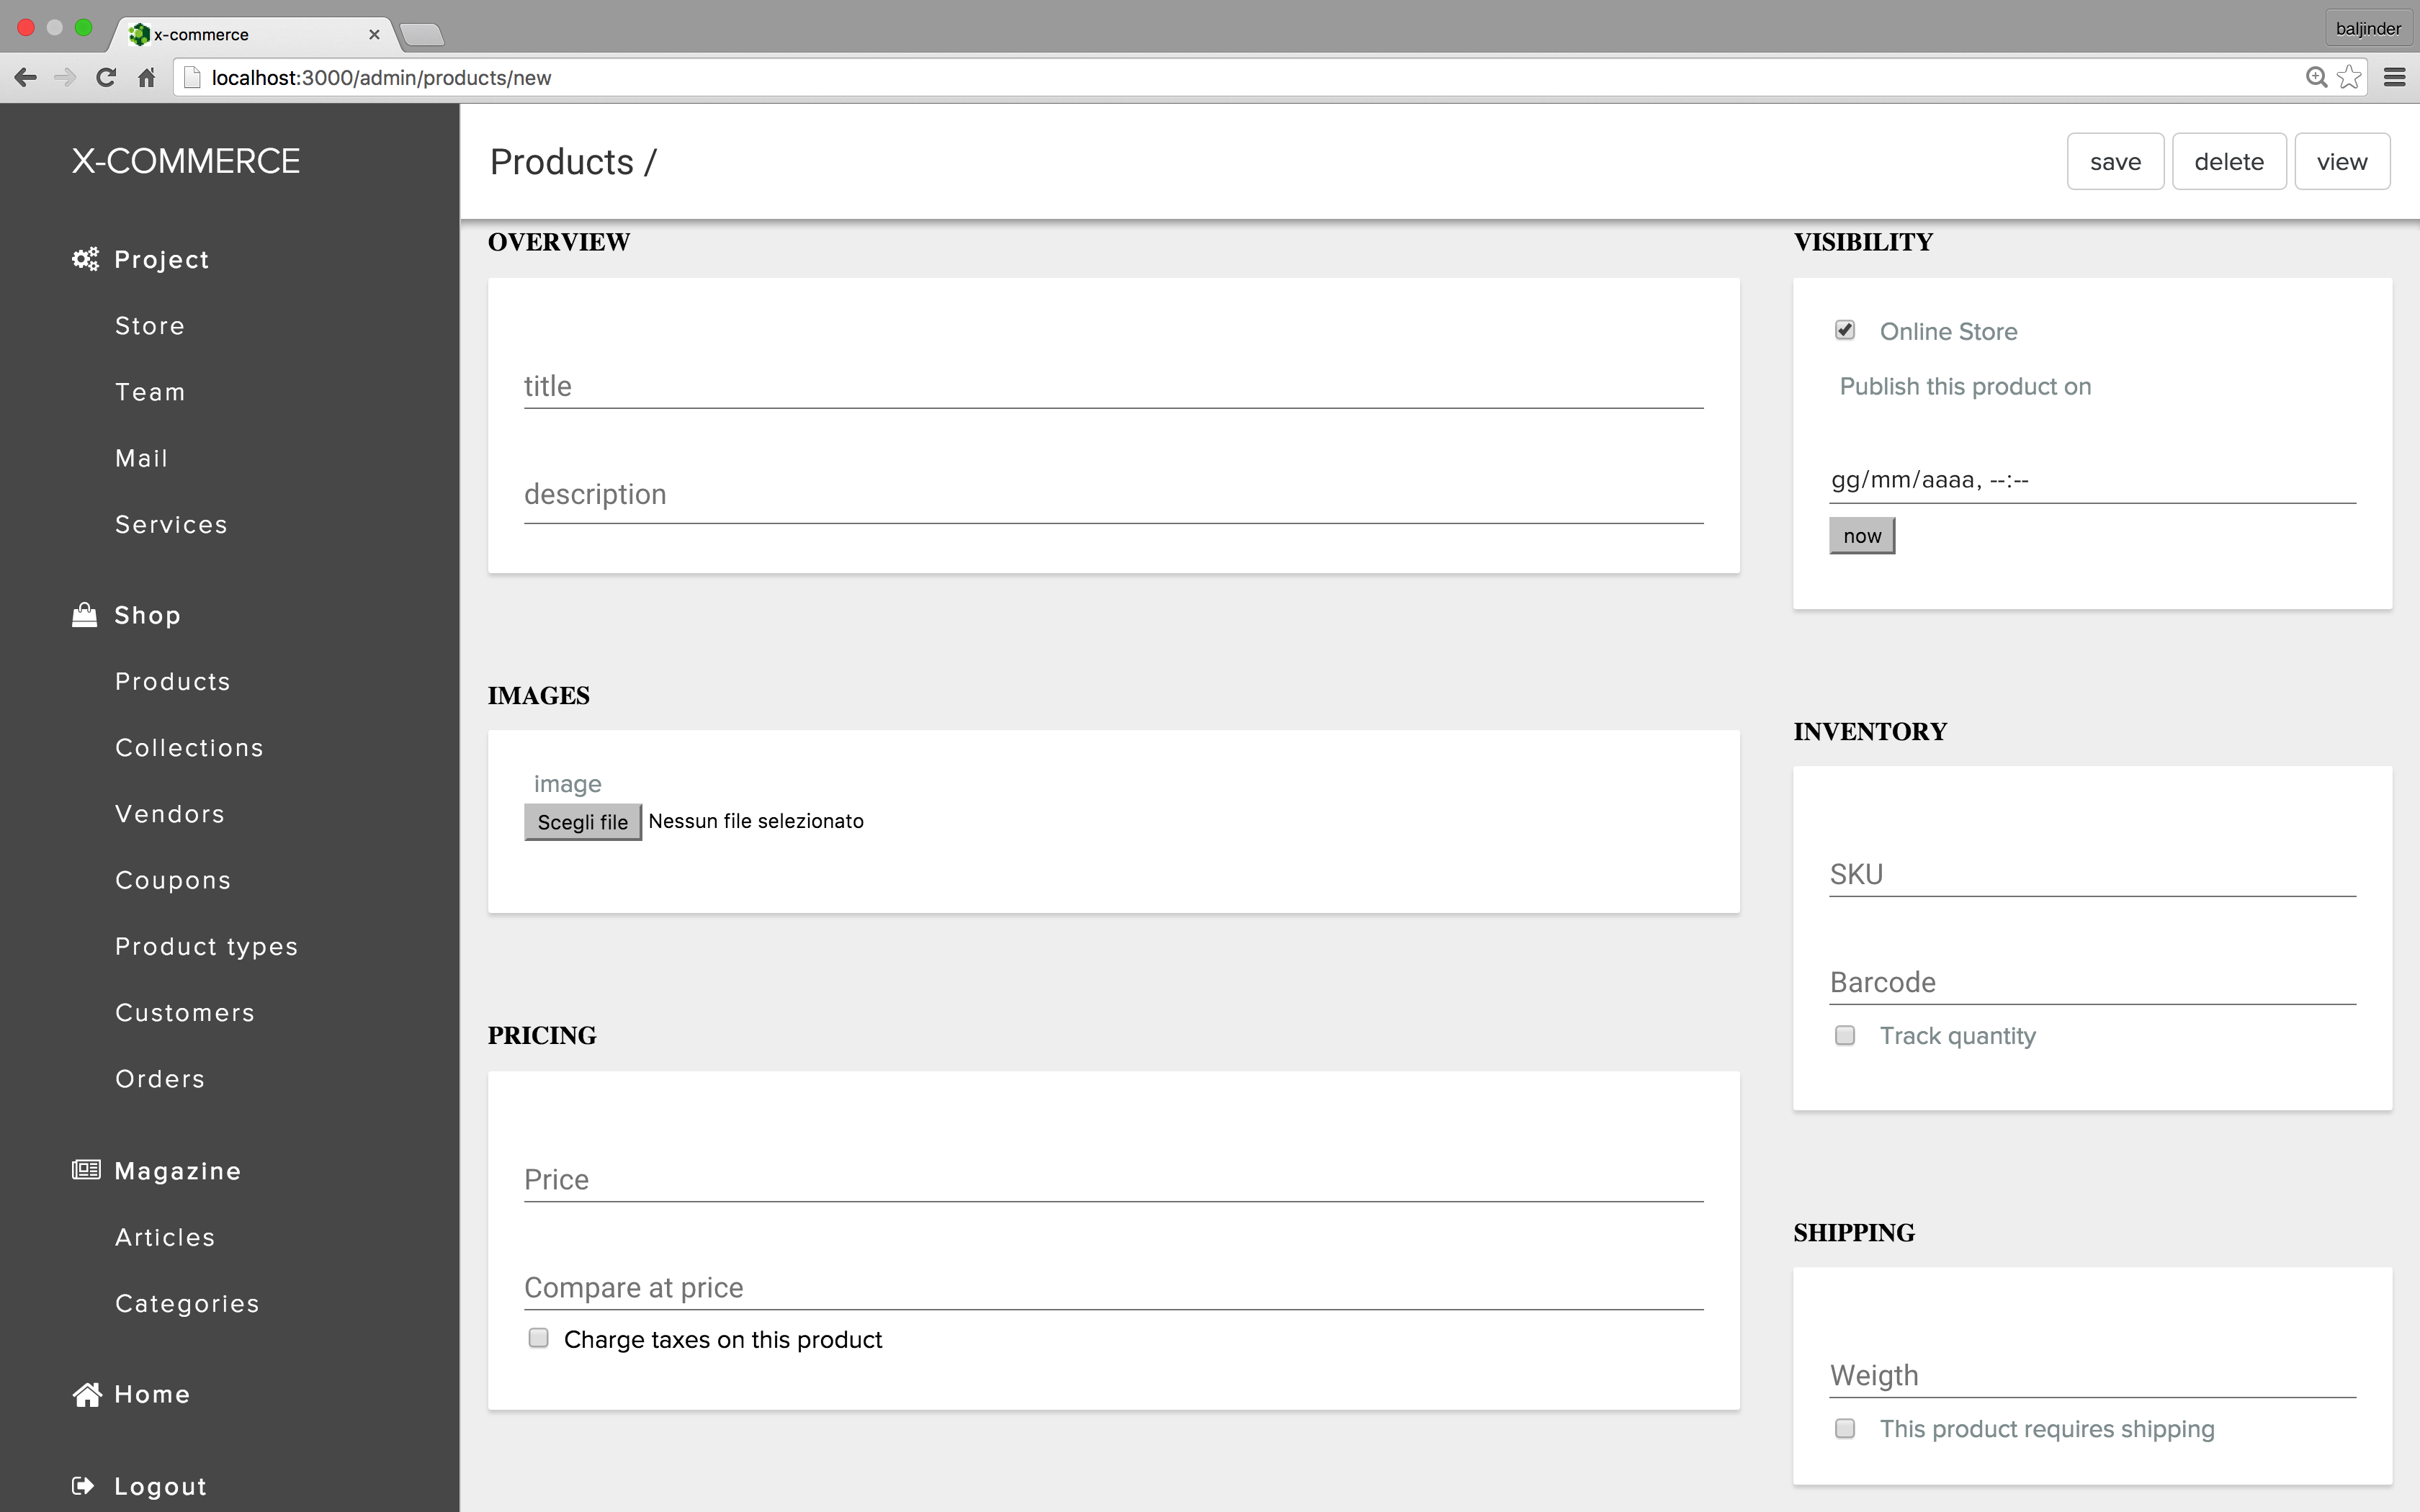
\includegraphics[width=1.0\linewidth]{images/chapter4/product-page-ex1.png}\hfill
\caption[Product page first part form]{Example for product page - first part forms interface}
\label{fig:design_page}
\end{figure}
\newline
This first part of the product page consists of several components:
\begin{itemize}
\item
\begin{lstlisting}[language=html]
<part-product-header></part-product-header>
\end{lstlisting}
this component is used to represent the \emph{breadcrumb} and buttons to perform the action on the product;
\item
\begin{lstlisting}[language=html]
<part-product-info></part-product-info>
\end{lstlisting}
this element manages information based on a product such as the name and description;
\item
\begin{lstlisting}[language=html]
<part-product-visibility></part-product-visibility>
\end{lstlisting}
this component serves to schedule the date of publication of the product on the store;
\item
\begin{lstlisting}[language=html]
<part-product-image></part-product-image>
\end{lstlisting}
this component is used to show the images of the product;
\end{itemize}
%second part of page product%
Following is shown a second part of the product page:
\begin{figure}[htb]
\centering
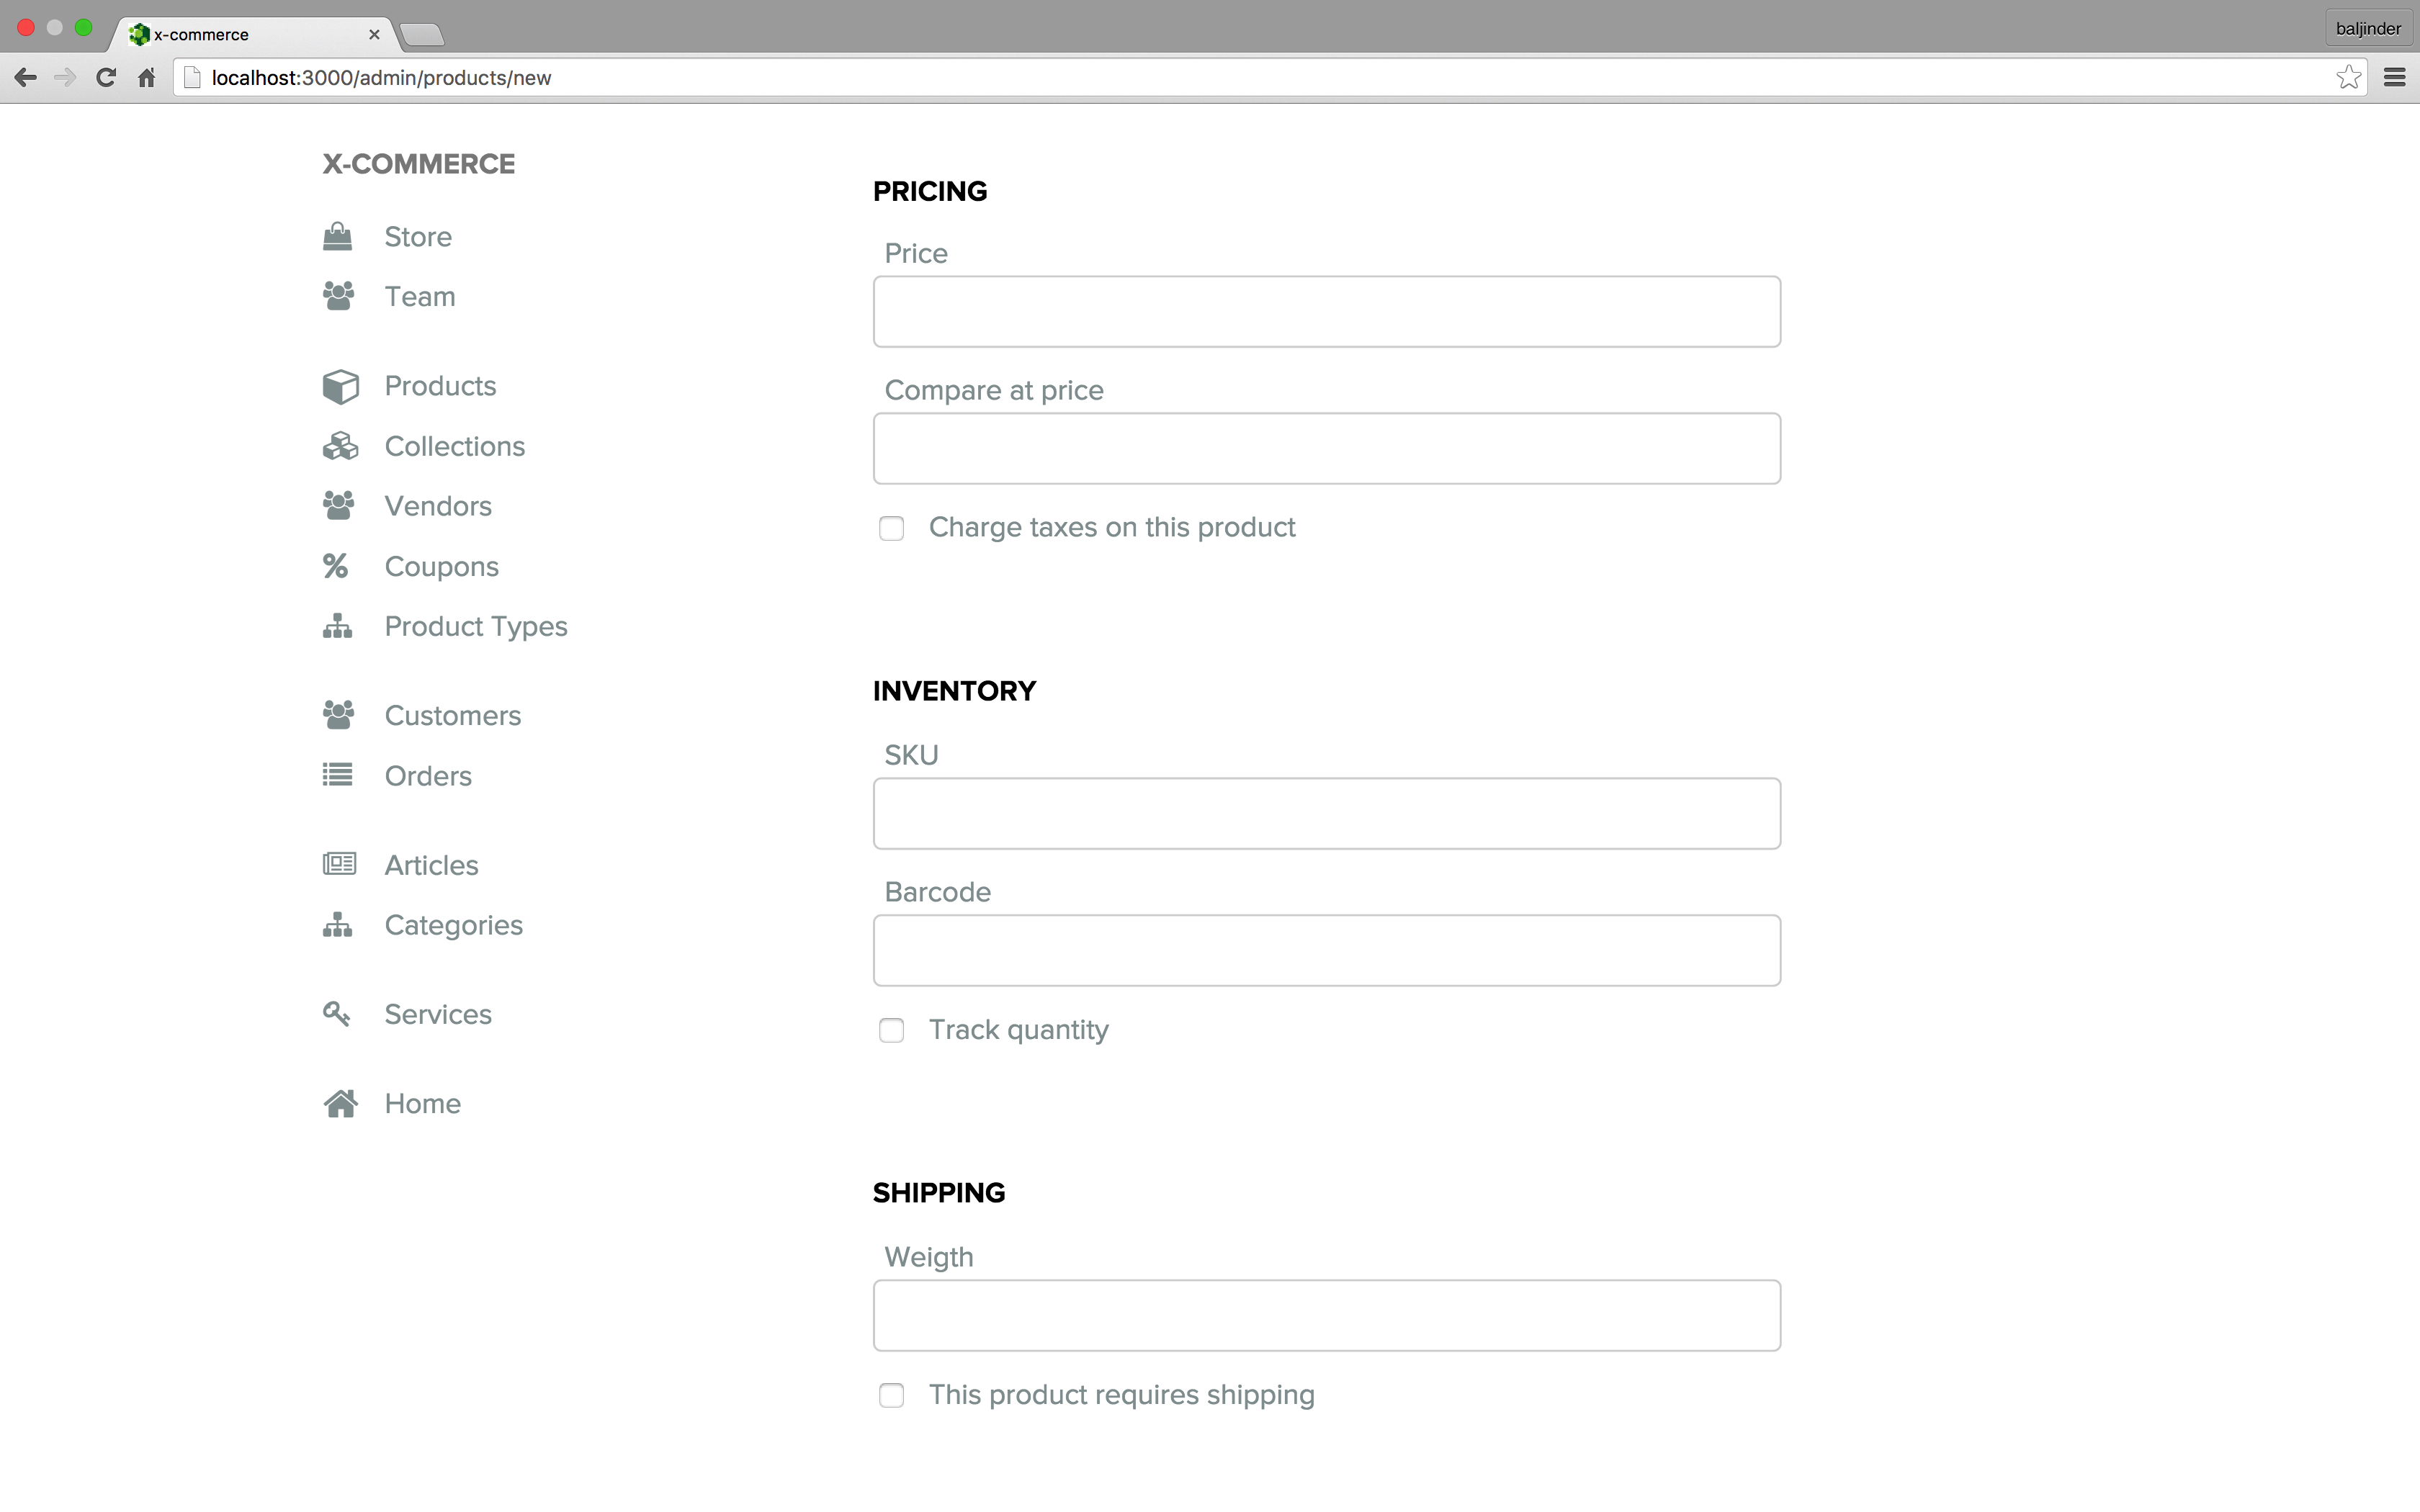
\includegraphics[width=0.9\linewidth]{images/chapter4/product-page-ex2.png}\hfill
\caption[Product page second part form]{Example for product page - second part forms interface}
\label{fig:design_page}
\end{figure}
\newline
This second part of the product page contains other components:
\begin{itemize}
\item
\begin{lstlisting}[language=html]
<part-product-pricing></part-product-pricing>
\end{lstlisting}
this component shows the information related to the price;
\item
\begin{lstlisting}[language=html]
<part-product-inventory></part-product-inventory>
\end{lstlisting}
this component is used to represents the information related to inventory as barcode and SKU(stock keeping unit);
\item
\begin{lstlisting}[language=html]
<part-product-shipping></part-product-shipping>
\end{lstlisting}
this component is used to indicate the weight of product;
\end{itemize}
%third part of page product%
Following is shown a third part of the product page:
\begin{figure}[htb]
\centering
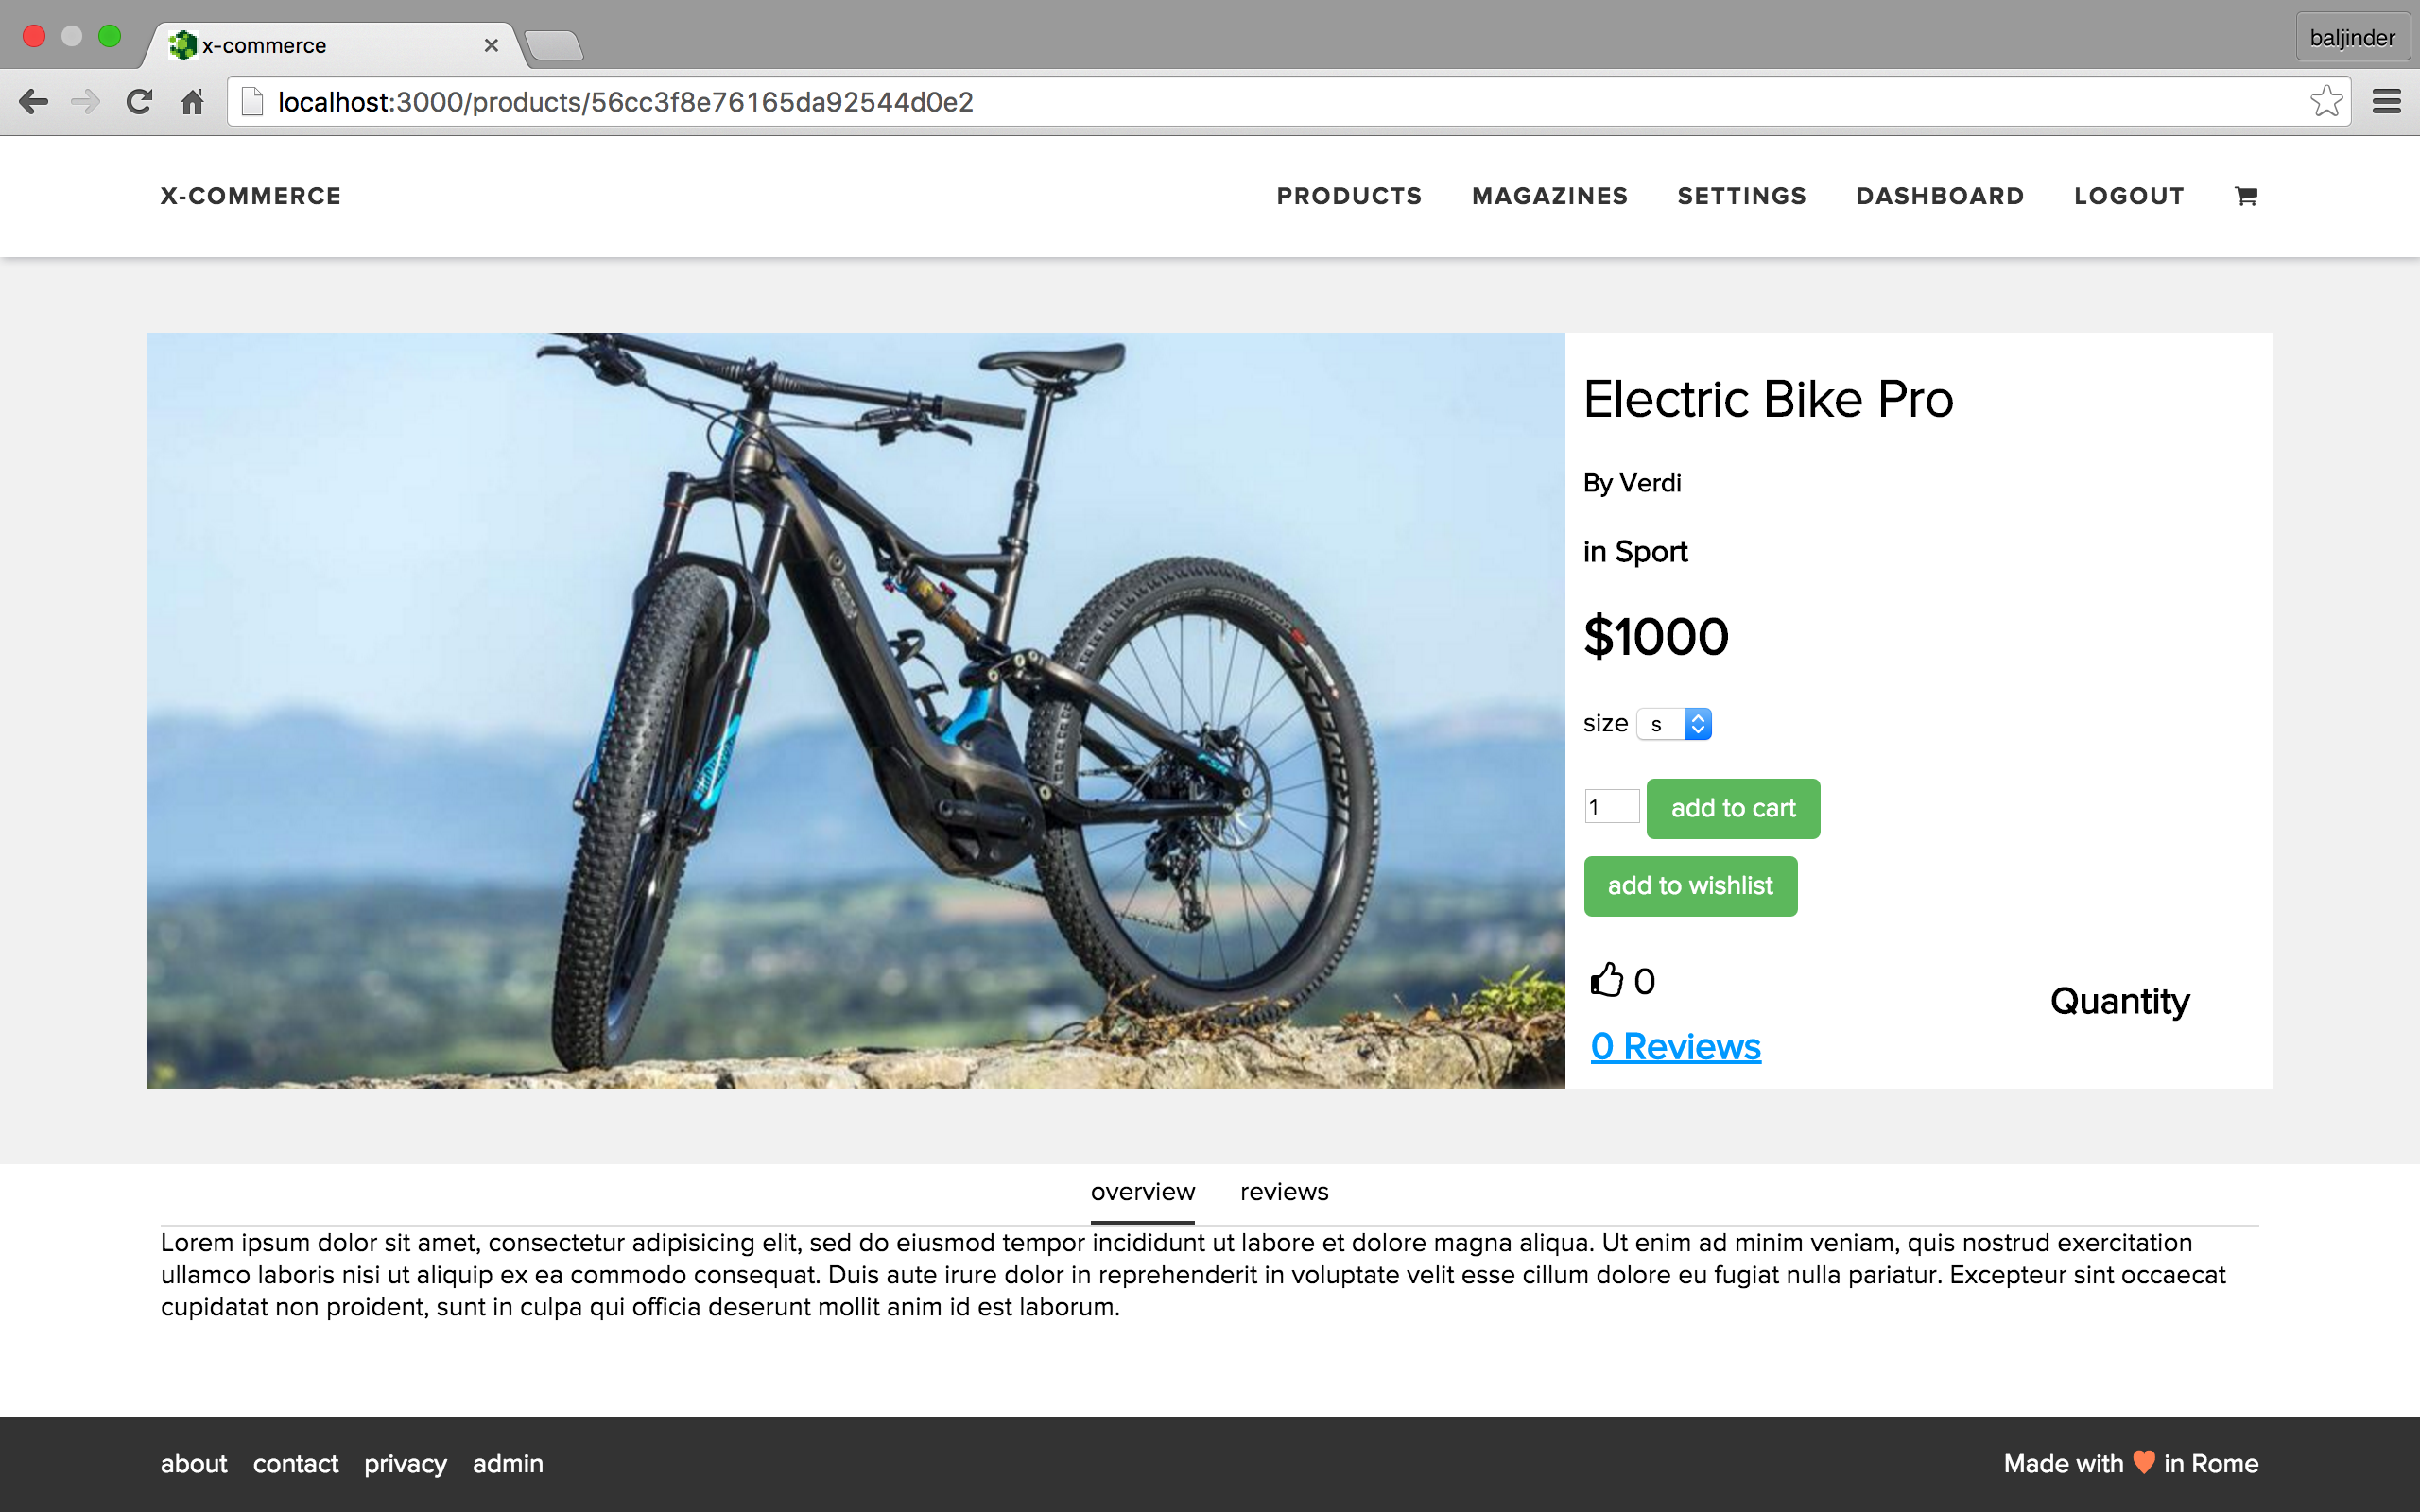
\includegraphics[width=1.0\linewidth]{images/chapter4/product-page-ex3.png}\hfill
\caption[Product page third part form]{Example for product page - third part forms interface}
\label{fig:design_page}
\end{figure}
\newline
This third part of the product page contains other components:
\begin{itemize}
\item
\begin{lstlisting}[language=html]
<part-product-organization></part-product-organization>
\end{lstlisting}
this component hides all the operating logic to assign the current product to a seller, to one or more collections, defines the type of product. Finally, it is possible to assign the tag to the product;
\item
\begin{lstlisting}[language=html]
<part-product-variants></part-product-variants>
\end{lstlisting}
this component hides the entire operating logic to create variants of a product;
\item
\begin{lstlisting}[language=html]
<part-product-actions></part-product-actions>
\end{lstlisting}
This component is the buttons of saving a product and its display at the client side;
\end{itemize}
Putting together these small self-contained components, the product page is designed. Now let us see how the product page at client-side it designed.
\subsubsection{Client side}
\begin{figure}[htb]
\centering
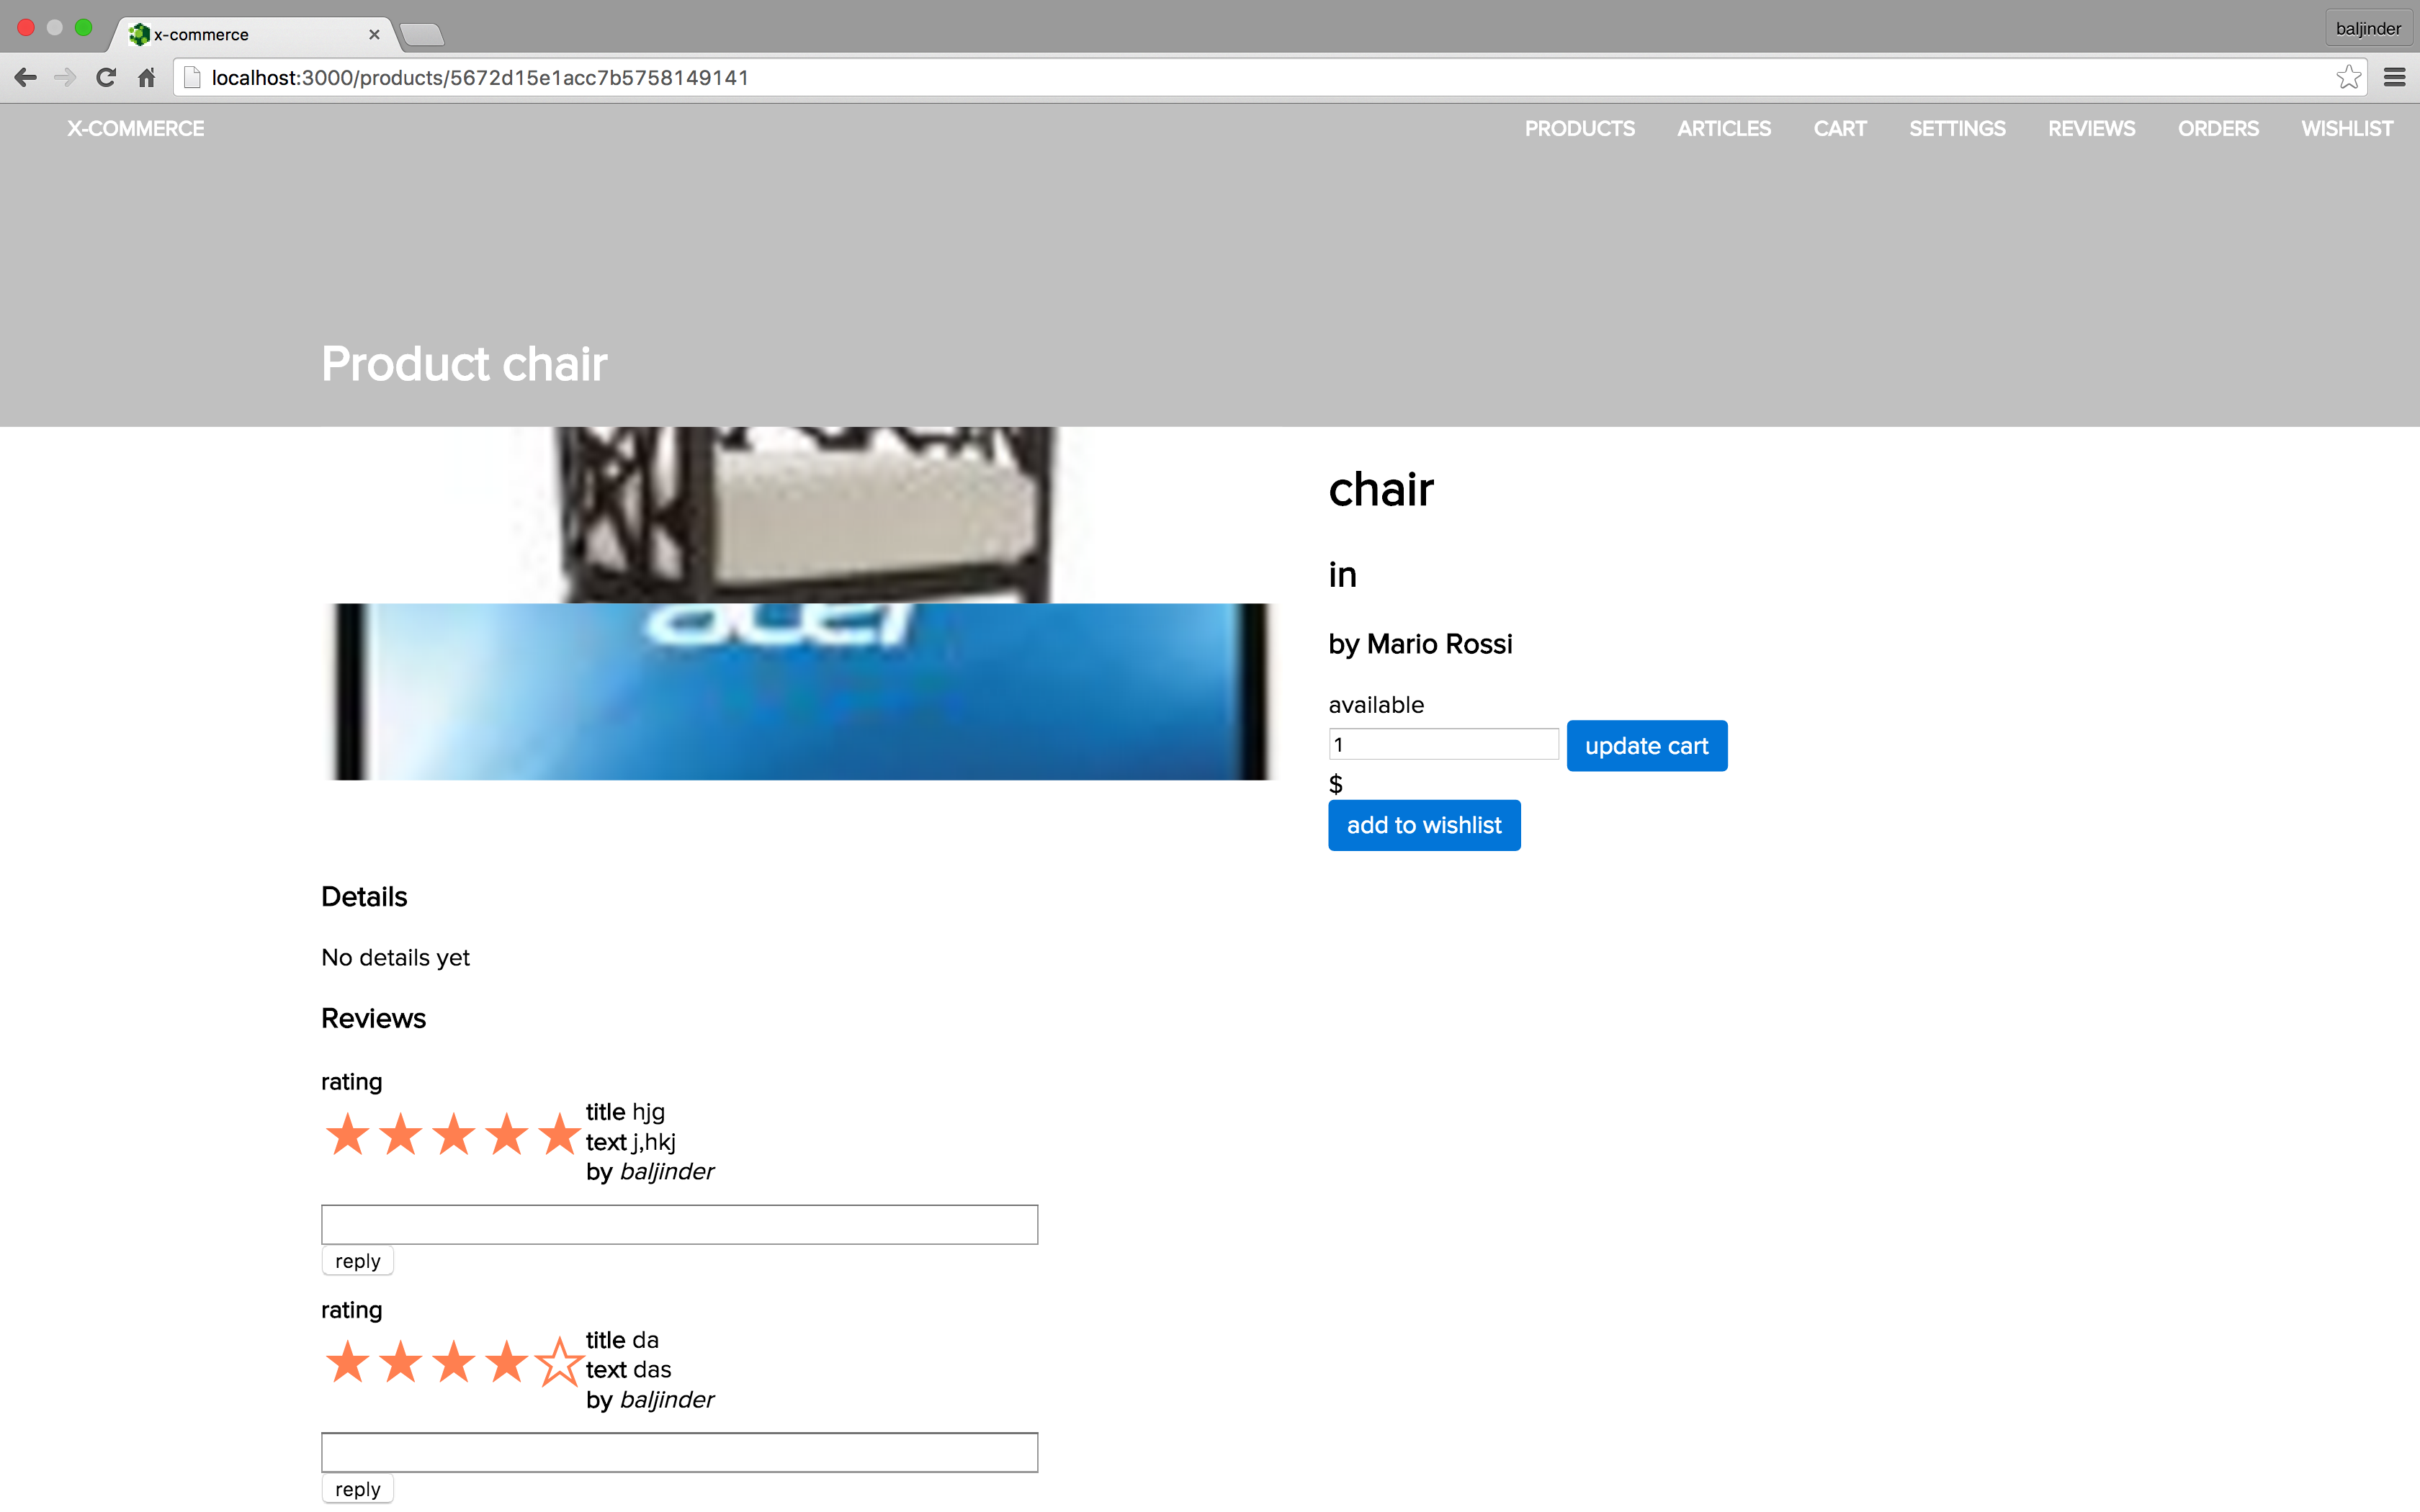
\includegraphics[width=0.9\linewidth]{images/chapter4/product-page-ex4.png}\hfill
\caption[Product page on client-side]{Product page on client-side example}
\label{fig:design_page_prod_cli}
\end{figure}
The components making up the product page on the client-side are as follows:
\begin{lstlisting}[language=html]
<part-product-info></part-product-info>
<part-product-options></part-product-options>
<part-product-cart></part-product-cart>
<part-product-wish></part-product-wish>
<part-product-details></part-product-details>
<part-product-reviews></part-product-reviews>
\end{lstlisting}
The role of each component in the page is made clear.

\chapter{Payment management}
\label{cha:payment_management}

A payment system is any system used to settle financial transactions through the transfer of monetary value, and includes the institutions, instruments, people, rules, procedures, standards, and technologies that make such an exchange possible.
\newline
What makes a payment system a system is the use of cash-substitutes; traditional payment systems are negotiable instruments such as drafts (e.g., checks) and documentary credits such as letters of credit. With the advent of computers and electronic communications a large number of alternative electronic payment systems have emerged. These include debit cards, credit cards, electronic funds transfers, direct credits, direct debits, internet banking and e-commerce payment systems.
\newline
Payment systems are used in lieu of tendering cash in domestic and international transactions and consist of a major service provided by banks and other financial institutions.
\newline
This chapter describes how the payment services are intgrated in x-commerce project. In particular, the first paragraph sets out some principal companies that provide services like payment service provider. In the following paragraphs we will enter more and more in detail in the use of these services.

\section{x-commerce payment system overview}
\label{sec:payment_system_overview}
In the management of payments of e-commerce, there are three major players involved:
\begin{itemize}
\item \emph{x-commmerce client}: it is the one who initiates the transaction. The customer enters their credit card details in the specific form and send those to the server of x-commerce;
\item \emph{x-commmerce server} the x-commerce server verifies the data received from the client and communicates with the server to start a transaction of Braintree;
\item \emph{Braintree server} The server braintree also called a “gateway” initiates the transaction on the basis of the coordinates of the credit card.
The needed results of the operation is sent to the server of x-commerce which in turn notifies the customer.
\end{itemize}
\subsection{Braintree customized form}
In section \ref{sec:braintree} shows how to set the base form provided by Braintree to integrate payments into your application. Following example shows the code to create a custom form:
\begin{lstlisting}[language=html]
<form action="/api/orders/checkout" id="form_card">
  <div>
    <label for="card-number">Card Number</label>
    <input type="text" data-braintree-name="number">
  </div>
  <div>
    <label for="expiration-date">Expiration Date</label>
    <input type="number" data-braintree-name="expiration_month">
    <input type="number" data-braintree-name="expiration_year">
  </div>
  <input id="pay" type="submit" value="pay">
</form>
<script src="https://js.braintreegateway.com/v2/braintree.js"></script>
<script>
  braintree.setup("YOUR_CLIENT_TOKEN", "custom", { id: "form_card" });
</script>
\end{lstlisting}
This way you can customize the form with CSS code.
Note that the first thing that comes to imported script \emph{braintree.js}.
This library includes all the logic for the management of sending data. In particular, the data on credit cards do not travel on the network as this script first hides such data with a token. Network so traveling a token that summarizes the data of the credit card. A server-side that is sufficient token to decode the token to get clear in the coordinates of the credit card. This token is generated from the keys and other information obtained from Braintree and is unique. In fact if you start two transactions and both have the same token then the second is discarded because it was considered duplicated.
Immediately after the values are dictated to the environment variable “braintree”.
\begin{lstlisting}[language=javascript]
<script>
  braintree.setup("YOUR_CLIENT_TOKEN", "custom", { id: "form_card" });
</script>
\end{lstlisting}
Where:
\begin{itemize}
\item \emph{YOUR\_CLIENT\_TOKEN}: it's the ID of braintree's client that get with an AJAX call. The customer must be registered in Braintree.
Braintree provides APIs to register a new account and get ID assigned to it;
\item \emph{custom}: it indicates that the form of payment is not the default (\emph{dropin}) but is customized;
\item \emph{id}: specific ID of the form that must be processed by the library \emph{braintree.js} to submit the form.
\end{itemize}
Finally the script \emph{braintree.js}, to process the data of credit cards, requires that each input field has certain characteristics.
\begin{lstlisting}[language=html]
<div>
<label for="card-number">Card Number</label>
<input type="text" data-braintree-name="number"></div>
<div>
<label for="expiration-date">Expiration Date</label>
<input type="number" data-braintree-name="expiration_month">
<input type="number" data-braintree-name="expiration_year">
</div>
\end{lstlisting}
Where:
\begin{itemize}
\item \emph{data-braintree-name="number"}: it's need to add this property to the input field of the form. This input field contains the number of the credit card that is used by the script \emph{braintree.js} to generate the token. This is necessary because the form is submitted, the script braintree.js parses the data entered in the form in particular select input fields having these specific properties;
\item \emph{data-braintree-name="expiration\_month"}: it's need to add this property to the input field of the form that will contain the month of expiration of the credit card;
\item \emph{data-braintree-name="expiration\_year"}: it's need to add this property to the input field of the form that will contain the year of expiration of the credit card.
\end{itemize}
So, in this way the customer x-commerce is able to send the data of the credit card to the server of x-commerce, then start a payment transaction.
\subsection{Payment transaction initialization - server side}
For initilize, the x-commerce server must import the Braintree di module.
This module must be initialized with the keys that uniquely identify the merchant.
\newline
These keys are obtained from braintree and are used to make authentication on Braintree and are the following:
\begin{itemize}
\item \emph{merchant ID}: identifies the merchant
\item \emph{public key}: It is the public key of the asymmetric encryption used in sending data from client to server;
\item \emph{private key}: It is the public key of the asymmetric encryption used to decrypt the data;
\end{itemize}
In the following is a function that, thanks to these keys, it connects to the gateway braintree:
\begin{lstlisting}[language=javascript]
  var gateway;
  function connect_braintree () {
    return new Promise(function (resolve, reject) {
      if (gateway) {
        resolve(gateway);
        return;
      }
      get_service('braintree').then(function (service) {
        gateway = braintree.connect({
          environment: braintree.Environment.Sandbox,
          merchantId: service.params.merchant_id,
          publicKey: service.public_key,
          privateKey: service.private_key
        });
        resolve(gateway);
      }).catch(function (err) {
        reject(err);
      });
    });
  }
\end{lstlisting}
In this way, through the variable \emph{gateway}, it is possible to communicate with braintree.
\newline
Once you are done with authentication braintree and received the token ( \emph{payment\_method\_none}), which summarizes the data of the credit card, one can try to make the payment.
\newline
When the customer does submit the payment form, it is chiamara API: \emph{/api/orders/checkout}.
At the call of this API, a server-side function is called \emph{checkout\_braintree}, which performs the following functions:
\begin{enumerate}
\item get the customer from his ID. A query is made to the database that returns the customer associated with the ID;
\item creation a new order as required by the customer. To do this, run a series of operations such as block related products due cause, occurs if the customer used a coupon, etc..;
\item communicates with braintree server for initilize a new payment trasction;
\item creating review to allow the customer to leave a review for each product order;
\item mark current order as closed;
\item save the response of Braintree to keep track of the attempted payment;
\item creation of a new bill to be sent to the customer;
\item save the data required to retry the payment in case the first attempt went wrong;
\item prepare response for showing to client;
\end{enumerate}
The point 3, as already said, start a new transaction to try the payment. Following example shows the code for this:
\begin{lstlisting}[language=javascript]
  var braintree_checkout = function (data) {
    return function (next) {
      connect_braintree().then(function (gateway) { // connects with Braintree server
        var sale_data = {
          amount: 1,
          paymentMethodNonce: data.payment_method_nonce,
          options: {
            submitForSettlement: true
          }
        };
        gateway.transaction.sale(sale_data, function (err, res) {
          next(err, res);
        );
      }).catch(function (err){
          next(err, null);
      });
    };
  };
\end{lstlisting}
Where:
\begin{enumerate}
\item connection with the server Braintree;
\item preparing payment data such as the amount, payment\_method\_nonce encoding information of the credit card use by the customer;
\item finally send payment;
\end{enumerate}
Once you send a payment, the following operations to be performed depend on the outcome of the transaction. In particular, if the transaction is successful then you must carry out steps 4, 5, 7, 8, 9 otherwise runs the operation of point 6 which repeats the whole procedure.
\newline
In the next section it describes in detail the operation that is performed in point 6.

{\color{red} -----------------------corretto il quarto capitolo fino a qui----------------------}
\section{Execute tasks to retry payment}
\label{sec:tasks_to_retry_payment}
The payment of an order can have different outcomes in particular:
\begin{itemize}
\item It can fail for the following reasons:
\begin{itemize}
\item error in data entry of credit card;
\item for network problems;
\item insufficient credit;
\item unknown reasons;
\end{itemize}
\item transaction successfully completed;
\end{itemize}
In each of these cases the customer e-commerce must be notified of the outcome of the transaction.
\newline
In the case in which the customer inserts the data of the credit card incorrect then it is immediately alerted.
\newline
If the data on the card are correct but there are other problems for which the first transaction fails to complete for reasons listed above, Braintree then returns a reply containing identifier of the failed transaction.
\newline
This transaction ID (and other information) is stored in the DB to retry payment in particular is used to store the template \emph{task} this information.
In particular, if a payment transaction fails then the server x-commerce creates a instance of the task model with the following data:
\begin{lstlisting}[language=javascript]
  var get_task_braintree = function (data) {
    var date_now = moment().format().split('+')[0] + 'Z';
    var task = {
      data: {
        order_id: data.order.id,
        transaction_id: data.payment_status.transaction.id,
        customer_id: data.customer.id,
        payment_system: 'braintree'
      },
      handler: 'retry_payment',
      created_at: date_now,
      priority: 'medium',
      last_retry_at: date_now,
      retry_count: 1,
      done: false
    };
    return task;
  };
\end{lstlisting}
When starts of x-commerce starts a cron that appropriate and regular intervals starts and checks if there are tasks to be performed.
A Cron is a time-based job scheduler in Unix-like computer operating systems.
The function of this scheduler is to verify the presence of tasks to be performed in particular:
\begin{itemize}
\item if there are no tasks to be performed then the crohn falls asleep;
\item if there are any cron task then it takes all tasks and we select a task to be carried out with a policy implemented in the following function:
\begin{lstlisting}[language=javascript]
  var get_next_task = function (tasks) {
    var test = false;
    var task = null;
    for(var i=0; i < tasks.length && !test; i++) {
      var last_retry_at = new Date(tasks[i].last_retry_at)
      var date_now = new Date(moment().format().split('+')[0] + 'Z');
      var minutes_past = (date_now - last_retry_at)/1000/60;
      if (minutes_past > Math.pow(tasks[i].retry_count, 4.09)) {
        task = tasks[i];
        test = true;
      }
    }
    return task;
  };
\end{lstlisting}
Selecting a task to perform depends on two main factors:\begin{itemize}
\item the number of attempts to retry the task;
\item the time since the last time the task was executed
\end{itemize}
In particular, the probability that a task is selected decreases as the number of attempts made for the task.
For example:
\begin{enumerate}
\item if a task with the retry\_count = 0 => \(0^{4,09} = 1\). Then this task is selected to run if it is spend at least one minute;
\item if a task with the retry\_count = 1 => \(1^{4,09} = 4,09\). Then this task is selected to run if they spent at least 4,09 minutes;
\item if a task with the retry\_count = 2 => \(2^{4,09} = 17,02\). Then this task is selected to run if they spent at least 17.02 minutes;
\item if a task with the retry\_count = 3 => \(3^{4,09} = 89,41\). Then this task is selected to run if they spent at least 89,41 minutes;
\item if a task with the retry\_count = 4 => \(4^{4,09} = 290,01\). Then this task is selected to run if they spent at least 290,01 minutes;
\end{enumerate}
As you can see, a new task is now selected to be tried again. Instead other tasks that continue to fail will gradually discarded.
\newline
This idea to try to make payment by executing the task is very important namely when the customer has entered the data of the credit card and did checkout then it is the responsibility of the administrator of the platform, the transaction was completed successfully without requiring the customer to try again.
\newline
This is appropriate because the customer could change his mind if you continue to ask him to refuse the payment. So it is advisable that the customer confirms the payment once only and all that needs to be managed at the server side.
\end{itemize}


\newpage

\chapter{Conclusions}
\label{cha:conclusions}

\section{Work performed}
\label{sec:work_performed}
In previous chapters we have seen the design and development of a web platform for the creation of a system of e-commerce.
\newline
The platform designed, X-commerce, has been realized with the newest technologies in both the client and server side.
\newline
As already mentioned, thanks to the Web components, the complexity of the project has been managed in separate and self-contained. In this way every element hides the operating logic and you can use it by simply inserting a tag on the page. This technique allows you to dial the complexity of the pages to define reusable elements.
\newline
Server-side benefits are represented by the easy way of API creation: describing procedures and model definitions are direct and can generate API and behavioural elements as well.
Finally, the union between server-side and client-side technologies allowed
to create vertical elements that cross all the architectural stack.
At the moment x-commerce, is the core of the e-commerce and implements the basic functions such as:
\begin{itemize}
\item insert, delete, update of new products, vendors, collections, coupons, product type, product options, etc ...
\item possibility to create, delete and manage the list of desires;
\item login with email and password;
\item login passwordless login via SMS and email;
\item possibility to generate variations of a product;
\item implements two payment systems: Braintree and Stripe;
\item implements the possibility to perform tasks in the event of a failure of some operation.
\item etc...
\end{itemize}

\section{Future developments}
\label{sec:future_work}
{\color{red}
X-commerce, allo stato attuale, offre un insieme di funzionalità di base per creare un applicazione di e-commerce e molte altre funzionalità richiedono di essere ancora sviluppate.
In particolare uno dei primi punti che vanno tra i sviluppi futuri è la creazione di un infrastruttura di deploy ovvero una applicazione responsabile di creare il negozio allocando opportuni server e attivazione di opportuni servizi al fine di fornire all'amministrare del negozio la possibilità di popolare e creare uno proprio store online.
\newline
Altri task altrettanto importanti e indispensabili che richiedono di essere sviluppati sono:
\begin{itemize}
\item integrazione di sistemi di shipping/tracking dei pacchi;
\item i temi giocano un ruolo molto importare in quanto rendono l'interfaccia utente flessibile e piacevole. Per questo, sviluppare un buon numero di temi, poterebbe aiutare x-commerce ad attirare più sviluppatori;
\item rendere la piattaforma ricca di eventi come ad esempio notificare ad un utente quanti altri utenti hanno fatto azioni simili. Predisposizione di una chat, possibilità di inviare email, blog, etc... renderebbe x-commerce più attirante e ricco di interrazioni;
\item integrare nuovi sistemi di pagamento oltre a quelli già esistenti (Braintree e Stripe);
\item generalizzare componenti fino a livello di pagina;
\item effettuare il porting da loopback a forester.js(si tratta di un framework sviluppato all'interno di CVDLAB che utilizza tecnologie che sono ancora in fase di sperimentazione);
\item portare applicazione su dispositivi mobile;
\end{itemize}
}


\newpage

\part{Appendix}

\appendix

\chapter{Appendix 1}
\label{cha:appendix_1}


In this appendix...

This is the appendix.

\chapter{Appendix 2}
\label{cha:appendix_2}


In this appendix...

This is the appendix.

\newpage

% BibTex

%\nocite{*}

% \bibliographystyle{ieeetr}

\cleardoublepage

\addcontentsline{toc}{chapter}{Bibliography}

\printbibliography

\input{tex_files/bibliography/bibliography}

\end{document}